
% Default to the notebook output style

    


% Inherit from the specified cell style.




    
\documentclass[11pt]{article}

    
    
    \usepackage[T1]{fontenc}
    % Nicer default font (+ math font) than Computer Modern for most use cases
    \usepackage{mathpazo}

    % Basic figure setup, for now with no caption control since it's done
    % automatically by Pandoc (which extracts ![](path) syntax from Markdown).
    \usepackage{graphicx}
    % We will generate all images so they have a width \maxwidth. This means
    % that they will get their normal width if they fit onto the page, but
    % are scaled down if they would overflow the margins.
    \makeatletter
    \def\maxwidth{\ifdim\Gin@nat@width>\linewidth\linewidth
    \else\Gin@nat@width\fi}
    \makeatother
    \let\Oldincludegraphics\includegraphics
    % Set max figure width to be 80% of text width, for now hardcoded.
    \renewcommand{\includegraphics}[1]{\Oldincludegraphics[width=.8\maxwidth]{#1}}
    % Ensure that by default, figures have no caption (until we provide a
    % proper Figure object with a Caption API and a way to capture that
    % in the conversion process - todo).
    \usepackage{caption}
    \DeclareCaptionLabelFormat{nolabel}{}
    \captionsetup{labelformat=nolabel}

    \usepackage{adjustbox} % Used to constrain images to a maximum size 
    \usepackage{xcolor} % Allow colors to be defined
    \usepackage{enumerate} % Needed for markdown enumerations to work
    \usepackage{geometry} % Used to adjust the document margins
    \usepackage{amsmath} % Equations
    \usepackage{amssymb} % Equations
    \usepackage{textcomp} % defines textquotesingle
    % Hack from http://tex.stackexchange.com/a/47451/13684:
    \AtBeginDocument{%
        \def\PYZsq{\textquotesingle}% Upright quotes in Pygmentized code
    }
    \usepackage{upquote} % Upright quotes for verbatim code
    \usepackage{eurosym} % defines \euro
    \usepackage[mathletters]{ucs} % Extended unicode (utf-8) support
    \usepackage[utf8x]{inputenc} % Allow utf-8 characters in the tex document
    \usepackage{fancyvrb} % verbatim replacement that allows latex
    \usepackage{grffile} % extends the file name processing of package graphics 
                         % to support a larger range 
    % The hyperref package gives us a pdf with properly built
    % internal navigation ('pdf bookmarks' for the table of contents,
    % internal cross-reference links, web links for URLs, etc.)
    \usepackage{hyperref}
    \usepackage{longtable} % longtable support required by pandoc >1.10
    \usepackage{booktabs}  % table support for pandoc > 1.12.2
    \usepackage[inline]{enumitem} % IRkernel/repr support (it uses the enumerate* environment)
    \usepackage[normalem]{ulem} % ulem is needed to support strikethroughs (\sout)
                                % normalem makes italics be italics, not underlines
    

    
    
    % Colors for the hyperref package
    \definecolor{urlcolor}{rgb}{0,.145,.698}
    \definecolor{linkcolor}{rgb}{.71,0.21,0.01}
    \definecolor{citecolor}{rgb}{.12,.54,.11}

    % ANSI colors
    \definecolor{ansi-black}{HTML}{3E424D}
    \definecolor{ansi-black-intense}{HTML}{282C36}
    \definecolor{ansi-red}{HTML}{E75C58}
    \definecolor{ansi-red-intense}{HTML}{B22B31}
    \definecolor{ansi-green}{HTML}{00A250}
    \definecolor{ansi-green-intense}{HTML}{007427}
    \definecolor{ansi-yellow}{HTML}{DDB62B}
    \definecolor{ansi-yellow-intense}{HTML}{B27D12}
    \definecolor{ansi-blue}{HTML}{208FFB}
    \definecolor{ansi-blue-intense}{HTML}{0065CA}
    \definecolor{ansi-magenta}{HTML}{D160C4}
    \definecolor{ansi-magenta-intense}{HTML}{A03196}
    \definecolor{ansi-cyan}{HTML}{60C6C8}
    \definecolor{ansi-cyan-intense}{HTML}{258F8F}
    \definecolor{ansi-white}{HTML}{C5C1B4}
    \definecolor{ansi-white-intense}{HTML}{A1A6B2}

    % commands and environments needed by pandoc snippets
    % extracted from the output of `pandoc -s`
    \providecommand{\tightlist}{%
      \setlength{\itemsep}{0pt}\setlength{\parskip}{0pt}}
    \DefineVerbatimEnvironment{Highlighting}{Verbatim}{commandchars=\\\{\}}
    % Add ',fontsize=\small' for more characters per line
    \newenvironment{Shaded}{}{}
    \newcommand{\KeywordTok}[1]{\textcolor[rgb]{0.00,0.44,0.13}{\textbf{{#1}}}}
    \newcommand{\DataTypeTok}[1]{\textcolor[rgb]{0.56,0.13,0.00}{{#1}}}
    \newcommand{\DecValTok}[1]{\textcolor[rgb]{0.25,0.63,0.44}{{#1}}}
    \newcommand{\BaseNTok}[1]{\textcolor[rgb]{0.25,0.63,0.44}{{#1}}}
    \newcommand{\FloatTok}[1]{\textcolor[rgb]{0.25,0.63,0.44}{{#1}}}
    \newcommand{\CharTok}[1]{\textcolor[rgb]{0.25,0.44,0.63}{{#1}}}
    \newcommand{\StringTok}[1]{\textcolor[rgb]{0.25,0.44,0.63}{{#1}}}
    \newcommand{\CommentTok}[1]{\textcolor[rgb]{0.38,0.63,0.69}{\textit{{#1}}}}
    \newcommand{\OtherTok}[1]{\textcolor[rgb]{0.00,0.44,0.13}{{#1}}}
    \newcommand{\AlertTok}[1]{\textcolor[rgb]{1.00,0.00,0.00}{\textbf{{#1}}}}
    \newcommand{\FunctionTok}[1]{\textcolor[rgb]{0.02,0.16,0.49}{{#1}}}
    \newcommand{\RegionMarkerTok}[1]{{#1}}
    \newcommand{\ErrorTok}[1]{\textcolor[rgb]{1.00,0.00,0.00}{\textbf{{#1}}}}
    \newcommand{\NormalTok}[1]{{#1}}
    
    % Additional commands for more recent versions of Pandoc
    \newcommand{\ConstantTok}[1]{\textcolor[rgb]{0.53,0.00,0.00}{{#1}}}
    \newcommand{\SpecialCharTok}[1]{\textcolor[rgb]{0.25,0.44,0.63}{{#1}}}
    \newcommand{\VerbatimStringTok}[1]{\textcolor[rgb]{0.25,0.44,0.63}{{#1}}}
    \newcommand{\SpecialStringTok}[1]{\textcolor[rgb]{0.73,0.40,0.53}{{#1}}}
    \newcommand{\ImportTok}[1]{{#1}}
    \newcommand{\DocumentationTok}[1]{\textcolor[rgb]{0.73,0.13,0.13}{\textit{{#1}}}}
    \newcommand{\AnnotationTok}[1]{\textcolor[rgb]{0.38,0.63,0.69}{\textbf{\textit{{#1}}}}}
    \newcommand{\CommentVarTok}[1]{\textcolor[rgb]{0.38,0.63,0.69}{\textbf{\textit{{#1}}}}}
    \newcommand{\VariableTok}[1]{\textcolor[rgb]{0.10,0.09,0.49}{{#1}}}
    \newcommand{\ControlFlowTok}[1]{\textcolor[rgb]{0.00,0.44,0.13}{\textbf{{#1}}}}
    \newcommand{\OperatorTok}[1]{\textcolor[rgb]{0.40,0.40,0.40}{{#1}}}
    \newcommand{\BuiltInTok}[1]{{#1}}
    \newcommand{\ExtensionTok}[1]{{#1}}
    \newcommand{\PreprocessorTok}[1]{\textcolor[rgb]{0.74,0.48,0.00}{{#1}}}
    \newcommand{\AttributeTok}[1]{\textcolor[rgb]{0.49,0.56,0.16}{{#1}}}
    \newcommand{\InformationTok}[1]{\textcolor[rgb]{0.38,0.63,0.69}{\textbf{\textit{{#1}}}}}
    \newcommand{\WarningTok}[1]{\textcolor[rgb]{0.38,0.63,0.69}{\textbf{\textit{{#1}}}}}
    
    
    % Define a nice break command that doesn't care if a line doesn't already
    % exist.
    \def\br{\hspace*{\fill} \\* }
    % Math Jax compatability definitions
    \def\gt{>}
    \def\lt{<}
    % Document parameters
    \title{10\_Histograms\_in\_OpenCV}
    
    
    

    % Pygments definitions
    
\makeatletter
\def\PY@reset{\let\PY@it=\relax \let\PY@bf=\relax%
    \let\PY@ul=\relax \let\PY@tc=\relax%
    \let\PY@bc=\relax \let\PY@ff=\relax}
\def\PY@tok#1{\csname PY@tok@#1\endcsname}
\def\PY@toks#1+{\ifx\relax#1\empty\else%
    \PY@tok{#1}\expandafter\PY@toks\fi}
\def\PY@do#1{\PY@bc{\PY@tc{\PY@ul{%
    \PY@it{\PY@bf{\PY@ff{#1}}}}}}}
\def\PY#1#2{\PY@reset\PY@toks#1+\relax+\PY@do{#2}}

\expandafter\def\csname PY@tok@w\endcsname{\def\PY@tc##1{\textcolor[rgb]{0.73,0.73,0.73}{##1}}}
\expandafter\def\csname PY@tok@c\endcsname{\let\PY@it=\textit\def\PY@tc##1{\textcolor[rgb]{0.25,0.50,0.50}{##1}}}
\expandafter\def\csname PY@tok@cp\endcsname{\def\PY@tc##1{\textcolor[rgb]{0.74,0.48,0.00}{##1}}}
\expandafter\def\csname PY@tok@k\endcsname{\let\PY@bf=\textbf\def\PY@tc##1{\textcolor[rgb]{0.00,0.50,0.00}{##1}}}
\expandafter\def\csname PY@tok@kp\endcsname{\def\PY@tc##1{\textcolor[rgb]{0.00,0.50,0.00}{##1}}}
\expandafter\def\csname PY@tok@kt\endcsname{\def\PY@tc##1{\textcolor[rgb]{0.69,0.00,0.25}{##1}}}
\expandafter\def\csname PY@tok@o\endcsname{\def\PY@tc##1{\textcolor[rgb]{0.40,0.40,0.40}{##1}}}
\expandafter\def\csname PY@tok@ow\endcsname{\let\PY@bf=\textbf\def\PY@tc##1{\textcolor[rgb]{0.67,0.13,1.00}{##1}}}
\expandafter\def\csname PY@tok@nb\endcsname{\def\PY@tc##1{\textcolor[rgb]{0.00,0.50,0.00}{##1}}}
\expandafter\def\csname PY@tok@nf\endcsname{\def\PY@tc##1{\textcolor[rgb]{0.00,0.00,1.00}{##1}}}
\expandafter\def\csname PY@tok@nc\endcsname{\let\PY@bf=\textbf\def\PY@tc##1{\textcolor[rgb]{0.00,0.00,1.00}{##1}}}
\expandafter\def\csname PY@tok@nn\endcsname{\let\PY@bf=\textbf\def\PY@tc##1{\textcolor[rgb]{0.00,0.00,1.00}{##1}}}
\expandafter\def\csname PY@tok@ne\endcsname{\let\PY@bf=\textbf\def\PY@tc##1{\textcolor[rgb]{0.82,0.25,0.23}{##1}}}
\expandafter\def\csname PY@tok@nv\endcsname{\def\PY@tc##1{\textcolor[rgb]{0.10,0.09,0.49}{##1}}}
\expandafter\def\csname PY@tok@no\endcsname{\def\PY@tc##1{\textcolor[rgb]{0.53,0.00,0.00}{##1}}}
\expandafter\def\csname PY@tok@nl\endcsname{\def\PY@tc##1{\textcolor[rgb]{0.63,0.63,0.00}{##1}}}
\expandafter\def\csname PY@tok@ni\endcsname{\let\PY@bf=\textbf\def\PY@tc##1{\textcolor[rgb]{0.60,0.60,0.60}{##1}}}
\expandafter\def\csname PY@tok@na\endcsname{\def\PY@tc##1{\textcolor[rgb]{0.49,0.56,0.16}{##1}}}
\expandafter\def\csname PY@tok@nt\endcsname{\let\PY@bf=\textbf\def\PY@tc##1{\textcolor[rgb]{0.00,0.50,0.00}{##1}}}
\expandafter\def\csname PY@tok@nd\endcsname{\def\PY@tc##1{\textcolor[rgb]{0.67,0.13,1.00}{##1}}}
\expandafter\def\csname PY@tok@s\endcsname{\def\PY@tc##1{\textcolor[rgb]{0.73,0.13,0.13}{##1}}}
\expandafter\def\csname PY@tok@sd\endcsname{\let\PY@it=\textit\def\PY@tc##1{\textcolor[rgb]{0.73,0.13,0.13}{##1}}}
\expandafter\def\csname PY@tok@si\endcsname{\let\PY@bf=\textbf\def\PY@tc##1{\textcolor[rgb]{0.73,0.40,0.53}{##1}}}
\expandafter\def\csname PY@tok@se\endcsname{\let\PY@bf=\textbf\def\PY@tc##1{\textcolor[rgb]{0.73,0.40,0.13}{##1}}}
\expandafter\def\csname PY@tok@sr\endcsname{\def\PY@tc##1{\textcolor[rgb]{0.73,0.40,0.53}{##1}}}
\expandafter\def\csname PY@tok@ss\endcsname{\def\PY@tc##1{\textcolor[rgb]{0.10,0.09,0.49}{##1}}}
\expandafter\def\csname PY@tok@sx\endcsname{\def\PY@tc##1{\textcolor[rgb]{0.00,0.50,0.00}{##1}}}
\expandafter\def\csname PY@tok@m\endcsname{\def\PY@tc##1{\textcolor[rgb]{0.40,0.40,0.40}{##1}}}
\expandafter\def\csname PY@tok@gh\endcsname{\let\PY@bf=\textbf\def\PY@tc##1{\textcolor[rgb]{0.00,0.00,0.50}{##1}}}
\expandafter\def\csname PY@tok@gu\endcsname{\let\PY@bf=\textbf\def\PY@tc##1{\textcolor[rgb]{0.50,0.00,0.50}{##1}}}
\expandafter\def\csname PY@tok@gd\endcsname{\def\PY@tc##1{\textcolor[rgb]{0.63,0.00,0.00}{##1}}}
\expandafter\def\csname PY@tok@gi\endcsname{\def\PY@tc##1{\textcolor[rgb]{0.00,0.63,0.00}{##1}}}
\expandafter\def\csname PY@tok@gr\endcsname{\def\PY@tc##1{\textcolor[rgb]{1.00,0.00,0.00}{##1}}}
\expandafter\def\csname PY@tok@ge\endcsname{\let\PY@it=\textit}
\expandafter\def\csname PY@tok@gs\endcsname{\let\PY@bf=\textbf}
\expandafter\def\csname PY@tok@gp\endcsname{\let\PY@bf=\textbf\def\PY@tc##1{\textcolor[rgb]{0.00,0.00,0.50}{##1}}}
\expandafter\def\csname PY@tok@go\endcsname{\def\PY@tc##1{\textcolor[rgb]{0.53,0.53,0.53}{##1}}}
\expandafter\def\csname PY@tok@gt\endcsname{\def\PY@tc##1{\textcolor[rgb]{0.00,0.27,0.87}{##1}}}
\expandafter\def\csname PY@tok@err\endcsname{\def\PY@bc##1{\setlength{\fboxsep}{0pt}\fcolorbox[rgb]{1.00,0.00,0.00}{1,1,1}{\strut ##1}}}
\expandafter\def\csname PY@tok@kc\endcsname{\let\PY@bf=\textbf\def\PY@tc##1{\textcolor[rgb]{0.00,0.50,0.00}{##1}}}
\expandafter\def\csname PY@tok@kd\endcsname{\let\PY@bf=\textbf\def\PY@tc##1{\textcolor[rgb]{0.00,0.50,0.00}{##1}}}
\expandafter\def\csname PY@tok@kn\endcsname{\let\PY@bf=\textbf\def\PY@tc##1{\textcolor[rgb]{0.00,0.50,0.00}{##1}}}
\expandafter\def\csname PY@tok@kr\endcsname{\let\PY@bf=\textbf\def\PY@tc##1{\textcolor[rgb]{0.00,0.50,0.00}{##1}}}
\expandafter\def\csname PY@tok@bp\endcsname{\def\PY@tc##1{\textcolor[rgb]{0.00,0.50,0.00}{##1}}}
\expandafter\def\csname PY@tok@fm\endcsname{\def\PY@tc##1{\textcolor[rgb]{0.00,0.00,1.00}{##1}}}
\expandafter\def\csname PY@tok@vc\endcsname{\def\PY@tc##1{\textcolor[rgb]{0.10,0.09,0.49}{##1}}}
\expandafter\def\csname PY@tok@vg\endcsname{\def\PY@tc##1{\textcolor[rgb]{0.10,0.09,0.49}{##1}}}
\expandafter\def\csname PY@tok@vi\endcsname{\def\PY@tc##1{\textcolor[rgb]{0.10,0.09,0.49}{##1}}}
\expandafter\def\csname PY@tok@vm\endcsname{\def\PY@tc##1{\textcolor[rgb]{0.10,0.09,0.49}{##1}}}
\expandafter\def\csname PY@tok@sa\endcsname{\def\PY@tc##1{\textcolor[rgb]{0.73,0.13,0.13}{##1}}}
\expandafter\def\csname PY@tok@sb\endcsname{\def\PY@tc##1{\textcolor[rgb]{0.73,0.13,0.13}{##1}}}
\expandafter\def\csname PY@tok@sc\endcsname{\def\PY@tc##1{\textcolor[rgb]{0.73,0.13,0.13}{##1}}}
\expandafter\def\csname PY@tok@dl\endcsname{\def\PY@tc##1{\textcolor[rgb]{0.73,0.13,0.13}{##1}}}
\expandafter\def\csname PY@tok@s2\endcsname{\def\PY@tc##1{\textcolor[rgb]{0.73,0.13,0.13}{##1}}}
\expandafter\def\csname PY@tok@sh\endcsname{\def\PY@tc##1{\textcolor[rgb]{0.73,0.13,0.13}{##1}}}
\expandafter\def\csname PY@tok@s1\endcsname{\def\PY@tc##1{\textcolor[rgb]{0.73,0.13,0.13}{##1}}}
\expandafter\def\csname PY@tok@mb\endcsname{\def\PY@tc##1{\textcolor[rgb]{0.40,0.40,0.40}{##1}}}
\expandafter\def\csname PY@tok@mf\endcsname{\def\PY@tc##1{\textcolor[rgb]{0.40,0.40,0.40}{##1}}}
\expandafter\def\csname PY@tok@mh\endcsname{\def\PY@tc##1{\textcolor[rgb]{0.40,0.40,0.40}{##1}}}
\expandafter\def\csname PY@tok@mi\endcsname{\def\PY@tc##1{\textcolor[rgb]{0.40,0.40,0.40}{##1}}}
\expandafter\def\csname PY@tok@il\endcsname{\def\PY@tc##1{\textcolor[rgb]{0.40,0.40,0.40}{##1}}}
\expandafter\def\csname PY@tok@mo\endcsname{\def\PY@tc##1{\textcolor[rgb]{0.40,0.40,0.40}{##1}}}
\expandafter\def\csname PY@tok@ch\endcsname{\let\PY@it=\textit\def\PY@tc##1{\textcolor[rgb]{0.25,0.50,0.50}{##1}}}
\expandafter\def\csname PY@tok@cm\endcsname{\let\PY@it=\textit\def\PY@tc##1{\textcolor[rgb]{0.25,0.50,0.50}{##1}}}
\expandafter\def\csname PY@tok@cpf\endcsname{\let\PY@it=\textit\def\PY@tc##1{\textcolor[rgb]{0.25,0.50,0.50}{##1}}}
\expandafter\def\csname PY@tok@c1\endcsname{\let\PY@it=\textit\def\PY@tc##1{\textcolor[rgb]{0.25,0.50,0.50}{##1}}}
\expandafter\def\csname PY@tok@cs\endcsname{\let\PY@it=\textit\def\PY@tc##1{\textcolor[rgb]{0.25,0.50,0.50}{##1}}}

\def\PYZbs{\char`\\}
\def\PYZus{\char`\_}
\def\PYZob{\char`\{}
\def\PYZcb{\char`\}}
\def\PYZca{\char`\^}
\def\PYZam{\char`\&}
\def\PYZlt{\char`\<}
\def\PYZgt{\char`\>}
\def\PYZsh{\char`\#}
\def\PYZpc{\char`\%}
\def\PYZdl{\char`\$}
\def\PYZhy{\char`\-}
\def\PYZsq{\char`\'}
\def\PYZdq{\char`\"}
\def\PYZti{\char`\~}
% for compatibility with earlier versions
\def\PYZat{@}
\def\PYZlb{[}
\def\PYZrb{]}
\makeatother


    % Exact colors from NB
    \definecolor{incolor}{rgb}{0.0, 0.0, 0.5}
    \definecolor{outcolor}{rgb}{0.545, 0.0, 0.0}



    
    % Prevent overflowing lines due to hard-to-break entities
    \sloppy 
    % Setup hyperref package
    \hypersetup{
      breaklinks=true,  % so long urls are correctly broken across lines
      colorlinks=true,
      urlcolor=urlcolor,
      linkcolor=linkcolor,
      citecolor=citecolor,
      }
    % Slightly bigger margins than the latex defaults
    
    \geometry{verbose,tmargin=1in,bmargin=1in,lmargin=1in,rmargin=1in}
    
    

    \begin{document}
    
    
    \maketitle
    
    

    
    \hypertarget{histograms-in-opencv}{%
\subsubsection{Histograms in OpenCV}\label{histograms-in-opencv}}

All about histograms in OpenCV

\hypertarget{histograms---1-find-plot-analyze}{%
\paragraph{Histograms - 1 : Find, Plot, Analyze
!!!}\label{histograms---1-find-plot-analyze}}

Learn the basics of histograms

\hypertarget{uxbaa9uxd45c}{%
\subparagraph{목표}\label{uxbaa9uxd45c}}

Learn to

\begin{itemize}
\tightlist
\item
  Find histograms, using both OpenCV and Numpy functions
\item
  Plot histograms, using OpenCV and Matplotlib functions
\item
  You will see these functions :
  \href{https://docs.opencv.org/3.4/d6/dc7/group__imgproc__hist.html\#ga4b2b5fd75503ff9e6844cc4dcdaed35d}{cv.calcHist()},
  np.histogram() etc.
\end{itemize}

\hypertarget{theory}{%
\subparagraph{Theory}\label{theory}}

그래서 히스토그램이란 무엇입니까? 히스토그램을 그래프 또는 플롯으로
생각하면 이미지의 강도 분포에 대한 전반적인 아이디어를 얻을 수 있습니다.
이것은 X 축에서 픽셀 값 (0에서 255까지의 범위, 항상은 아님)과 Y 축의
이미지에서 해당 픽셀 수를 갖는 플롯입니다.

이것은 이미지를 이해하는 또 다른 방법 일뿐입니다. 이미지의 히스토그램을
보면 이미지의 대비, 밝기, 강도 분포 등에 대한 직감을 얻을 수 있습니다.
오늘날 거의 모든 이미지 처리 도구는 히스토그램에 기능을 제공합니다.
아래는 Cambridge in Color 웹 사이트 의 이미지입니다 . 자세한 내용은 해당
사이트를 방문하시기 바랍니다

\includegraphics{https://docs.opencv.org/3.4/histogram_sample.jpg}
이미지와 그 히스토그램을 볼 수 있습니다. 이 히스토그램은 컬러 이미지가
아닌 회색 음영 이미지에 사용됩니다. 히스토그램의 왼쪽 영역은 이미지에서
어두운 픽셀의 양을 표시하고 오른쪽 영역은 밝은 픽셀의 양을 보여줍니다.
히스토그램을 보면 어두운 영역이 밝은 영역 이상이고 중간 톤 (중간 범위의
픽셀 값, 약 127 정도)의 양이 매우 적음을 알 수 있습니다.

\hypertarget{uxd788uxc2a4uxd1a0uxadf8uxb7a8-uxcc3euxae30}{%
\subparagraph{히스토그램
찾기}\label{uxd788uxc2a4uxd1a0uxadf8uxb7a8-uxcc3euxae30}}

이제 우리는 히스토그램이 무엇인지에 대한 아이디어를 얻었습니다.이를
어떻게 찾을 수 있는지 살펴볼 수 있습니다. OpenCV와 Numpy 모두이 기능을
내장하고 있습니다. 이러한 함수를 사용하기 전에 히스토그램과 관련된
용어를 이해해야합니다.

\textbf{BINS} : 위의 히스토그램은 모든 픽셀 값의 픽셀 수를 보여줍니다.
즉, 0에서 255까지입니다. 즉 위의 히스토그램을 표시하려면 256 개의 값이
필요합니다. 그러나 모든 픽셀 값의 픽셀 수를 따로 따로 구하지 않고 픽셀
값 간격의 픽셀 수를 찾을 필요가 없다면 어떻게할까요? 예를 들어, 0에서
15, 16에서 31, \ldots{}, 240에서 255 사이의 픽셀 수를 찾아야합니다.
히스토그램을 표시하려면 16 개의 값만 필요합니다. 그리고 그것은
히스토그램에 대한 OpenCV 자습서에 제공된 예제에 표시된 것입니다 .

그래서 당신은 단순히 전체 히스토그램을 16 개의 하위 파트로 나누고 각
하위 파트의 값은 모든 하위 픽셀의 합계입니다. 이 각 하위 부분을
``BIN''이라고합니다. 첫 번째 경우 빈의 수는 256 개 (각 픽셀 당 하나) 두
번째 경우는 16 개입니다 . \textbf{BINS} 는 OpenCV 문서에서
\textbf{histSize} 라는 용어로 표현됩니다 .

\textbf{DIMS} : 우리가 데이터를 수집하는 매개 변수의 수입니다. 이 경우,
우리는 단지 하나의 것, 강도 값에 관한 데이터를 수집합니다. 그래서 여기에
1입니다.

범위 : 측정하려는 강도 값의 범위입니다. 일반적으로 그것은 {[}0,256{]},
즉 모든 강도 값입니다.

1.OpenCV의 히스토그램 계산

이제 cv.calcHist () 함수를 사용 하여 히스토그램을 찾습니다. 함수와 매개
변수에 익숙해 지자.

\begin{quote}
cv.calcHist(images, channels, mask, histSize, ranges{[}, hist{[},
accumulate{]}{]})
\end{quote}

\begin{enumerate}
\def\labelenumi{\arabic{enumi}.}
\tightlist
\item
  images : uint8 또는 float32 유형의 소스 이미지입니다. 대괄호 (
  ``{[}img{]}'')로 표시해야합니다.
\item
  채널 : 대괄호 안에도 표시됩니다. 히스토그램을 계산하는 채널의
  인덱스입니다. 예를 들어 입력이 회색 명암 이미지 인 경우 그 값은
  {[}0{]}입니다. 컬러 이미지의 경우 {[}0{]}, {[}1{]} 또는 {[}2{]}를
  전달하여 청색, 녹색 또는 적색 채널의 히스토그램을 각각 계산할 수
  있습니다.
\item
  마스크 : 마스크 이미지. 전체 이미지의 막대 그래프를 찾으려면
  ``없음''으로 표시됩니다. 그러나 특정 이미지 영역의 히스토그램을
  찾으려면 마스크 이미지를 만들어 마스크로 제공해야합니다. (나중에
  예제를 보여줄 것입니다.)
\item
  histSize : BIN 수를 나타냅니다. 대괄호로 묶여 있어야합니다. 풀
  스케일의 경우 {[}256{]}을 전달합니다.
\item
  범위 : 이것이 우리 범위입니다. 일반적으로 {[}0,256{]}입니다.
\end{enumerate}

먼저 샘플 이미지부터 시작해 보겠습니다. 그레이 스케일 모드로
이미지를로드하고 전체 히스토그램을 찾으십시오.

2. Numpy에서의 히스토그램 계산

Numpy는 또한 np.histogram () 함수를 제공합니다 . 따라서 calcHist () 함수
대신 다음 줄을 시도해 볼 수 있습니다

    \begin{Verbatim}[commandchars=\\\{\}]
{\color{incolor}In [{\color{incolor}2}]:} \PY{k+kn}{import} \PY{n+nn}{cv2} \PY{k}{as} \PY{n+nn}{cv}
        \PY{k+kn}{import} \PY{n+nn}{numpy} \PY{k}{as} \PY{n+nn}{np}
        \PY{k+kn}{from} \PY{n+nn}{matplotlib} \PY{k}{import} \PY{n}{pyplot} \PY{k}{as} \PY{n}{plt}
        
        \PY{n}{img}  \PY{o}{=} \PY{n}{cv}\PY{o}{.}\PY{n}{imread}\PY{p}{(}\PY{l+s+s1}{\PYZsq{}}\PY{l+s+s1}{home.jpg}\PY{l+s+s1}{\PYZsq{}}\PY{p}{,} \PY{l+m+mi}{0}\PY{p}{)}
        \PY{n}{hist} \PY{o}{=} \PY{n}{cv}\PY{o}{.}\PY{n}{calcHist}\PY{p}{(}\PY{p}{[}\PY{n}{img}\PY{p}{]}\PY{p}{,} \PY{p}{[}\PY{l+m+mi}{0}\PY{p}{]}\PY{p}{,} \PY{k+kc}{None} \PY{p}{,} \PY{p}{[}\PY{l+m+mi}{256}\PY{p}{]}\PY{p}{,} \PY{p}{[}\PY{l+m+mi}{0}\PY{p}{,} \PY{l+m+mi}{256}\PY{p}{]}\PY{p}{)}
        \PY{n}{hist\PYZus{}np}\PY{p}{,} \PY{n}{bins} \PY{o}{=} \PY{n}{np}\PY{o}{.}\PY{n}{histogram}\PY{p}{(}\PY{n}{img}\PY{o}{.}\PY{n}{ravel}\PY{p}{(}\PY{p}{)}\PY{p}{,} \PY{l+m+mi}{256}\PY{p}{,} \PY{p}{[}\PY{l+m+mi}{0}\PY{p}{,} \PY{l+m+mi}{256}\PY{p}{]}\PY{p}{)}
\end{Verbatim}


    hist는 이전에 계산 한 것과 같습니다. 그러나 Numpy가 0-0.99, 1-1.99,
2-2.99 등으로 쓰레기를 계산하기 때문에 쓰레기통에 257 개의 요소가
있습니다. 따라서 최종 범위는 255-255.99가됩니다. 이를 나타 내기 위해 빈
끝에 256을 추가합니다. 하지만 우리는 256을 필요로하지 않습니다.
255까지는 충분합니다.

또한보십시오 Numpy는 또 다른 함수 인 np.bincount () 를 사용합니다 (약 10
배) np.histogram ()보다 훨씬 빠릅니다. 따라서 1 차원 히스토그램의 경우
더 잘 시도 할 수 있습니다. np.bincount에 minlength = 256을 설정하는 것을
잊지 마십시오. 예를 들어, hist = np.bincount (img.ravel (), minlength =
256) 노트 OpenCV 함수는 np.histogram ()보다 (약 40X) 빠릅니다. 그래서
OpenCV 기능을 고수하십시오. 이제 우리는 히스토그램을 계획해야하지만
어떻게해야합니까?

\hypertarget{uxd788uxc2a4uxd1a0uxadf8uxb7a8-uxadf8uxb9acuxae30}{%
\subparagraph{히스토그램
그리기}\label{uxd788uxc2a4uxd1a0uxadf8uxb7a8-uxadf8uxb9acuxae30}}

이 방법에는 두 가지가 있습니다.

짧은 길 : Matplotlib 플로팅 함수 사용 긴 방법 : OpenCV 그리기 기능 사용

1. Matplotlib 사용하기

Matplotlib에는 히스토그램 플롯 기능이 있습니다 : matplotlib.pyplot.hist
()

히스토그램을 직접 찾아서 그려줍니다. 히스토그램을 찾으려면
\textbf{calcHist()} 또는 \textbf{np.histogram()} 함수를 사용할 필요가
없습니다 . 아래 코드를 참조하십시오.

    \begin{Verbatim}[commandchars=\\\{\}]
{\color{incolor}In [{\color{incolor}3}]:} \PY{n}{plt}\PY{o}{.}\PY{n}{hist}\PY{p}{(}\PY{n}{img}\PY{o}{.}\PY{n}{ravel}\PY{p}{(}\PY{p}{)}\PY{p}{,}\PY{l+m+mi}{256}\PY{p}{,}\PY{p}{[}\PY{l+m+mi}{0}\PY{p}{,}\PY{l+m+mi}{256}\PY{p}{]}\PY{p}{)}
        \PY{n}{plt}\PY{o}{.}\PY{n}{show}\PY{p}{(}\PY{p}{)}
\end{Verbatim}


    \begin{center}
    \adjustimage{max size={0.9\linewidth}{0.9\paperheight}}{output_3_0.png}
    \end{center}
    { \hspace*{\fill} \\}
    
    또는 matplotlib의 일반 플롯을 사용할 수 있습니다.이 플롯은 BGR 플롯에
유용합니다. 이를 위해서는 히스토그램 데이터를 먼저 찾아야합니다. 아래
코드를 시도하십시오.

    \begin{Verbatim}[commandchars=\\\{\}]
{\color{incolor}In [{\color{incolor}4}]:} \PY{k+kn}{import} \PY{n+nn}{numpy} \PY{k}{as} \PY{n+nn}{np}
        \PY{k+kn}{import} \PY{n+nn}{cv2} \PY{k}{as} \PY{n+nn}{cv}
        \PY{k+kn}{from} \PY{n+nn}{matplotlib} \PY{k}{import} \PY{n}{pyplot} \PY{k}{as} \PY{n}{plt}
        
        \PY{n}{img} \PY{o}{=} \PY{n}{cv}\PY{o}{.}\PY{n}{imread}\PY{p}{(}\PY{l+s+s1}{\PYZsq{}}\PY{l+s+s1}{home.jpg}\PY{l+s+s1}{\PYZsq{}}\PY{p}{)}
        \PY{n}{color} \PY{o}{=} \PY{p}{(}\PY{l+s+s1}{\PYZsq{}}\PY{l+s+s1}{b}\PY{l+s+s1}{\PYZsq{}}\PY{p}{,}\PY{l+s+s1}{\PYZsq{}}\PY{l+s+s1}{g}\PY{l+s+s1}{\PYZsq{}}\PY{p}{,}\PY{l+s+s1}{\PYZsq{}}\PY{l+s+s1}{r}\PY{l+s+s1}{\PYZsq{}}\PY{p}{)}
        
        \PY{k}{for} \PY{n}{i}\PY{p}{,}\PY{n}{col} \PY{o+ow}{in} \PY{n+nb}{enumerate}\PY{p}{(}\PY{n}{color}\PY{p}{)}\PY{p}{:}
            \PY{n}{histr} \PY{o}{=} \PY{n}{cv}\PY{o}{.}\PY{n}{calcHist}\PY{p}{(}\PY{p}{[}\PY{n}{img}\PY{p}{]}\PY{p}{,} \PY{p}{[}\PY{n}{i}\PY{p}{]}\PY{p}{,} \PY{k+kc}{None}\PY{p}{,} \PY{p}{[}\PY{l+m+mi}{256}\PY{p}{]}\PY{p}{,} \PY{p}{[}\PY{l+m+mi}{0}\PY{p}{,}\PY{l+m+mi}{256}\PY{p}{]}\PY{p}{)}
            \PY{n}{plt}\PY{o}{.}\PY{n}{plot}\PY{p}{(}\PY{n}{histr}\PY{p}{,}\PY{n}{color} \PY{o}{=} \PY{n}{col}\PY{p}{)}
            \PY{n}{plt}\PY{o}{.}\PY{n}{xlim}\PY{p}{(}\PY{p}{[}\PY{l+m+mi}{0}\PY{p}{,} \PY{l+m+mi}{256}\PY{p}{]}\PY{p}{)}
        \PY{n}{plt}\PY{o}{.}\PY{n}{show}\PY{p}{(}\PY{p}{)}
\end{Verbatim}


    \begin{center}
    \adjustimage{max size={0.9\linewidth}{0.9\paperheight}}{output_5_0.png}
    \end{center}
    { \hspace*{\fill} \\}
    
    2. OpenCV 사용하기

여기서 히스토그램의 값을 bin 값과 함께 x, y 좌표와 같이 조정하여 cv.line
() 또는 cv.polyline () 함수를 사용하여 위와 동일한 이미지를 생성 할 수
있습니다 . 이것은 OpenCV-Python2 공식 샘플에서 이미 사용 가능합니다.
samples / python / hist.py의 코드를 확인하십시오.

    \begin{Verbatim}[commandchars=\\\{\}]
{\color{incolor}In [{\color{incolor}15}]:} \PY{o}{\PYZpc{}}\PY{k}{run} hist.py
\end{Verbatim}


    \begin{Verbatim}[commandchars=\\\{\}]
usage : python hist.py <image\_file>
 Histogram plotting 

    Keymap :

    a - show histogram for color image in curve mode 

    b - show histogram in bin mode 

    c - show equalized histogram (always in bin mode) 

    d - show histogram for color image in curve mode 

    e - show histogram for a normalized image in curve mode 

    Esc - exit 

    
a
a
b
hist\_lines applicable only for grayscale images
c
d
e
a
b
hist\_lines applicable only for grayscale images
c
d
e
a
b
hist\_lines applicable only for grayscale images
c
d
e
a
b
hist\_lines applicable only for grayscale images
c
d
e
ESC

    \end{Verbatim}

    
    \begin{verbatim}
<Figure size 432x288 with 0 Axes>
    \end{verbatim}

    
    \hypertarget{uxb9c8uxc2a4uxd06c-uxc801uxc6a9}{%
\subparagraph{마스크 적용}\label{uxb9c8uxc2a4uxd06c-uxc801uxc6a9}}

cv.calcHist () 를 사용 하여 전체 이미지의 히스토그램을 찾습니다.
이미지의 일부 영역에 대한 히스토그램을 찾고 싶다면 어떻게해야할까요?
히스토그램을 찾으려는 영역에 흰색으로 마스크 이미지를 만들고 그렇지
않으면 검정색으로 만듭니다. 그런 다음 이것을 마스크로 전달하십시오.

    \begin{Verbatim}[commandchars=\\\{\}]
{\color{incolor}In [{\color{incolor}8}]:} \PY{k+kn}{import} \PY{n+nn}{cv2} \PY{k}{as} \PY{n+nn}{cv}
        \PY{k+kn}{import} \PY{n+nn}{numpy} \PY{k}{as} \PY{n+nn}{np}
        \PY{k+kn}{from} \PY{n+nn}{matplotlib} \PY{k}{import} \PY{n}{pyplot} \PY{k}{as} \PY{n}{plt}
        
        \PY{n}{img} \PY{o}{=} \PY{n}{cv}\PY{o}{.}\PY{n}{imread}\PY{p}{(}\PY{l+s+s1}{\PYZsq{}}\PY{l+s+s1}{home.jpg}\PY{l+s+s1}{\PYZsq{}}\PY{p}{,}\PY{l+m+mi}{0}\PY{p}{)}
        
        \PY{c+c1}{\PYZsh{} create a mask}
        \PY{n}{mask} \PY{o}{=} \PY{n}{np}\PY{o}{.}\PY{n}{zeros}\PY{p}{(}\PY{n}{img}\PY{o}{.}\PY{n}{shape}\PY{p}{[}\PY{p}{:}\PY{l+m+mi}{2}\PY{p}{]}\PY{p}{,} \PY{n}{np}\PY{o}{.}\PY{n}{uint8}\PY{p}{)}
        \PY{n}{mask}\PY{p}{[}\PY{l+m+mi}{100}\PY{p}{:}\PY{l+m+mi}{348}\PY{p}{,} \PY{l+m+mi}{100}\PY{p}{:}\PY{l+m+mi}{890}\PY{p}{]} \PY{o}{=} \PY{l+m+mi}{255}
        \PY{n}{masked\PYZus{}img} \PY{o}{=} \PY{n}{cv}\PY{o}{.}\PY{n}{bitwise\PYZus{}and}\PY{p}{(}\PY{n}{img}\PY{p}{,}\PY{n}{img}\PY{p}{,}\PY{n}{mask} \PY{o}{=} \PY{n}{mask}\PY{p}{)}
        
        \PY{c+c1}{\PYZsh{} Calculate histogram with mask and without mask}
        \PY{c+c1}{\PYZsh{} Check third argument for mask}
        \PY{n}{hist\PYZus{}full} \PY{o}{=} \PY{n}{cv}\PY{o}{.}\PY{n}{calcHist}\PY{p}{(}\PY{p}{[}\PY{n}{img}\PY{p}{]}\PY{p}{,} \PY{p}{[}\PY{l+m+mi}{0}\PY{p}{]}\PY{p}{,} \PY{k+kc}{None}\PY{p}{,} \PY{p}{[}\PY{l+m+mi}{256}\PY{p}{]}\PY{p}{,} \PY{p}{[}\PY{l+m+mi}{0}\PY{p}{,}\PY{l+m+mi}{256}\PY{p}{]}\PY{p}{)}
        \PY{n}{hist\PYZus{}mask} \PY{o}{=} \PY{n}{cv}\PY{o}{.}\PY{n}{calcHist}\PY{p}{(}\PY{p}{[}\PY{n}{img}\PY{p}{]}\PY{p}{,} \PY{p}{[}\PY{l+m+mi}{0}\PY{p}{]}\PY{p}{,} \PY{n}{mask}\PY{p}{,} \PY{p}{[}\PY{l+m+mi}{256}\PY{p}{]}\PY{p}{,} \PY{p}{[}\PY{l+m+mi}{0}\PY{p}{,}\PY{l+m+mi}{256}\PY{p}{]}\PY{p}{)}
        \PY{n}{plt}\PY{o}{.}\PY{n}{subplot}\PY{p}{(}\PY{l+m+mi}{221}\PY{p}{)}\PY{p}{,} \PY{n}{plt}\PY{o}{.}\PY{n}{imshow}\PY{p}{(}\PY{n}{img}\PY{p}{,} \PY{l+s+s1}{\PYZsq{}}\PY{l+s+s1}{gray}\PY{l+s+s1}{\PYZsq{}}\PY{p}{)}
        \PY{n}{plt}\PY{o}{.}\PY{n}{subplot}\PY{p}{(}\PY{l+m+mi}{222}\PY{p}{)}\PY{p}{,} \PY{n}{plt}\PY{o}{.}\PY{n}{imshow}\PY{p}{(}\PY{n}{mask}\PY{p}{,}\PY{l+s+s1}{\PYZsq{}}\PY{l+s+s1}{gray}\PY{l+s+s1}{\PYZsq{}}\PY{p}{)}
        \PY{n}{plt}\PY{o}{.}\PY{n}{subplot}\PY{p}{(}\PY{l+m+mi}{223}\PY{p}{)}\PY{p}{,} \PY{n}{plt}\PY{o}{.}\PY{n}{imshow}\PY{p}{(}\PY{n}{masked\PYZus{}img}\PY{p}{,} \PY{l+s+s1}{\PYZsq{}}\PY{l+s+s1}{gray}\PY{l+s+s1}{\PYZsq{}}\PY{p}{)}
        \PY{n}{plt}\PY{o}{.}\PY{n}{subplot}\PY{p}{(}\PY{l+m+mi}{224}\PY{p}{)}\PY{p}{,} \PY{n}{plt}\PY{o}{.}\PY{n}{plot}\PY{p}{(}\PY{n}{hist\PYZus{}full}\PY{p}{)}\PY{p}{,} \PY{n}{plt}\PY{o}{.}\PY{n}{plot}\PY{p}{(}\PY{n}{hist\PYZus{}mask}\PY{p}{)}
        \PY{n}{plt}\PY{o}{.}\PY{n}{xlim}\PY{p}{(}\PY{p}{[}\PY{l+m+mi}{0}\PY{p}{,}\PY{l+m+mi}{256}\PY{p}{]}\PY{p}{)}
        \PY{n}{plt}\PY{o}{.}\PY{n}{show}\PY{p}{(}\PY{p}{)}
\end{Verbatim}


    \begin{center}
    \adjustimage{max size={0.9\linewidth}{0.9\paperheight}}{output_9_0.png}
    \end{center}
    { \hspace*{\fill} \\}
    
    \hypertarget{additional-resources}{%
\subparagraph{Additional Resources}\label{additional-resources}}

\begin{enumerate}
\def\labelenumi{\arabic{enumi}.}
\tightlist
\item
  \href{http://www.cambridgeincolour.com/tutorials/histograms1.htm}{Cambridge
  in Color website}
\end{enumerate}

\hypertarget{exercises}{%
\subparagraph{Exercises}\label{exercises}}

    \hypertarget{histograms---2-histogram-equalization}{%
\paragraph{Histograms - 2: Histogram
Equalization}\label{histograms---2-histogram-equalization}}

히스토그램을 평준화하여 이미지의 대비를 향상시키는 방법 배우기

\hypertarget{uxbaa9uxd45c}{%
\subparagraph{목표}\label{uxbaa9uxd45c}}

In this section,

We will learn the concepts of histogram equalization and use it to
improve the contrast of our images.

\hypertarget{thory}{%
\subparagraph{Thory}\label{thory}}

픽셀 값이 특정 값 범위에만 국한되어있는 이미지를 생각해보십시오. 예를
들어, 밝은 이미지의 경우 모든 픽셀이 높은 값으로 제한됩니다. 그러나 좋은
이미지는 이미지의 모든 영역에서 픽셀을 갖습니다. 따라서이 히스토그램을
어느 한쪽 끝까지 늘려야합니다 (아래 이미지, 위키 피 디아에서 제공됨).
이것이 바로 히스토그램 이퀄라이제이션입니다 (간단한 단어로). 이렇게하면
일반적으로 이미지의 대비가 향상됩니다.

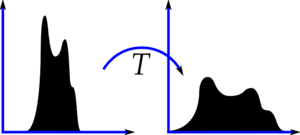
\includegraphics{histogram_equalization.png}

그것에 대한 자세한 내용은
\href{https://en.wikipedia.org/wiki/Histogram_equalization}{히스토그램
이퀄라이제이션 (Histogram Equalization)}에 대한 위키피디아 페이지를 읽어
보길 권합니다 . 그것은 잘 읽은 예제를 가지고 아주 잘 설명되어 있습니다.
그래서 그것을 읽은 후에 거의 모든 것을 이해할 수 있습니다. 대신 여기
Numpy 구현을 볼 것입니다. 그 다음에는 OpenCV 기능이 표시됩니다.

    \begin{Verbatim}[commandchars=\\\{\}]
{\color{incolor}In [{\color{incolor}9}]:} \PY{k+kn}{import} \PY{n+nn}{numpy} \PY{k}{as} \PY{n+nn}{np}
        \PY{k+kn}{import} \PY{n+nn}{cv2} \PY{k}{as} \PY{n+nn}{cv}
        \PY{k+kn}{from} \PY{n+nn}{matplotlib} \PY{k}{import} \PY{n}{pyplot} \PY{k}{as} \PY{n}{plt}
        \PY{o}{\PYZpc{}}\PY{k}{matplotlib} inline
        
        \PY{n}{img} \PY{o}{=} \PY{n}{cv}\PY{o}{.}\PY{n}{imread}\PY{p}{(}\PY{l+s+s1}{\PYZsq{}}\PY{l+s+s1}{wiki.jpg}\PY{l+s+s1}{\PYZsq{}}\PY{p}{,} \PY{l+m+mi}{0}\PY{p}{)}
        
        \PY{n}{hist}\PY{p}{,} \PY{n}{bins}      \PY{o}{=} \PY{n}{np}\PY{o}{.}\PY{n}{histogram}\PY{p}{(}\PY{n}{img}\PY{o}{.}\PY{n}{flatten}\PY{p}{(}\PY{p}{)}\PY{p}{,} \PY{l+m+mi}{256}\PY{p}{,} \PY{p}{[}\PY{l+m+mi}{0}\PY{p}{,} \PY{l+m+mi}{256}\PY{p}{]}\PY{p}{)}
        \PY{n}{cdf}             \PY{o}{=} \PY{n}{hist}\PY{o}{.}\PY{n}{cumsum}\PY{p}{(}\PY{p}{)}
        \PY{n}{cdf\PYZus{}normalized}  \PY{o}{=} \PY{n}{cdf} \PY{o}{*} \PY{n+nb}{float}\PY{p}{(}\PY{n}{hist}\PY{o}{.}\PY{n}{max}\PY{p}{(}\PY{p}{)}\PY{p}{)} \PY{o}{/} \PY{n}{cdf}\PY{o}{.}\PY{n}{max}\PY{p}{(}\PY{p}{)}
        
        
        \PY{n}{plt}\PY{o}{.}\PY{n}{plot}\PY{p}{(}\PY{n}{cdf\PYZus{}normalized}\PY{p}{,} \PY{n}{color} \PY{o}{=} \PY{l+s+s1}{\PYZsq{}}\PY{l+s+s1}{b}\PY{l+s+s1}{\PYZsq{}}\PY{p}{)}
        \PY{n}{plt}\PY{o}{.}\PY{n}{hist}\PY{p}{(}\PY{n}{img}\PY{o}{.}\PY{n}{flatten}\PY{p}{(}\PY{p}{)}\PY{p}{,} \PY{l+m+mi}{256}\PY{p}{,} \PY{p}{[}\PY{l+m+mi}{0}\PY{p}{,} \PY{l+m+mi}{256}\PY{p}{]}\PY{p}{,} \PY{n}{color} \PY{o}{=} \PY{l+s+s1}{\PYZsq{}}\PY{l+s+s1}{r}\PY{l+s+s1}{\PYZsq{}}\PY{p}{)}
        \PY{n}{plt}\PY{o}{.}\PY{n}{xlim}\PY{p}{(}\PY{p}{[}\PY{l+m+mi}{0}\PY{p}{,} \PY{l+m+mi}{256}\PY{p}{]}\PY{p}{)}
        \PY{n}{plt}\PY{o}{.}\PY{n}{legend}\PY{p}{(}\PY{p}{(}\PY{l+s+s1}{\PYZsq{}}\PY{l+s+s1}{cdf}\PY{l+s+s1}{\PYZsq{}}\PY{p}{,} \PY{l+s+s1}{\PYZsq{}}\PY{l+s+s1}{histogram}\PY{l+s+s1}{\PYZsq{}}\PY{p}{)}\PY{p}{,} \PY{n}{loc} \PY{o}{=} \PY{l+s+s1}{\PYZsq{}}\PY{l+s+s1}{upper left}\PY{l+s+s1}{\PYZsq{}}\PY{p}{)}
        \PY{n}{plt}\PY{o}{.}\PY{n}{show}\PY{p}{(}\PY{p}{)}
\end{Verbatim}


    \begin{center}
    \adjustimage{max size={0.9\linewidth}{0.9\paperheight}}{output_12_0.png}
    \end{center}
    { \hspace*{\fill} \\}
    
    밝은 영역에서 히스토그램 거짓을 볼 수 있습니다. 우리는 전체 스펙트럼이
필요합니다. 이를 위해 더 밝은 영역의 입력 픽셀을 전체 영역의 출력 픽셀에
매핑하는 변환 함수가 필요합니다. 그것이 히스토그램 평준화가하는
것입니다.

이제 우리는 최소 히스토그램 값 (0 제외)을 찾고 wiki 페이지에 주어진
히스토그램 등화 방정식을 적용합니다. 하지만 여기서 Numpy의 가면을 쓴
배열 개념 배열을 사용했습니다. 마스크 된 배열의 경우 모든 작업은
마스크가 적용되지 않은 요소에 대해 수행됩니다. 마스크 된 배열의 Numpy
문서에서 자세한 내용을 읽을 수 있습니다.

    \begin{Verbatim}[commandchars=\\\{\}]
{\color{incolor}In [{\color{incolor}10}]:} \PY{n}{cdf\PYZus{}m} \PY{o}{=} \PY{n}{np}\PY{o}{.}\PY{n}{ma}\PY{o}{.}\PY{n}{masked\PYZus{}equal}\PY{p}{(}\PY{n}{cdf}\PY{p}{,} \PY{l+m+mi}{0}\PY{p}{)}
         \PY{n}{cdf\PYZus{}m} \PY{o}{=} \PY{p}{(}\PY{n}{cdf\PYZus{}m} \PY{o}{\PYZhy{}} \PY{n}{cdf\PYZus{}m}\PY{o}{.}\PY{n}{min}\PY{p}{(}\PY{p}{)}\PY{p}{)} \PY{o}{*} \PY{l+m+mi}{255} \PY{o}{/} \PY{p}{(}\PY{n}{cdf\PYZus{}m}\PY{o}{.}\PY{n}{max}\PY{p}{(}\PY{p}{)} \PY{o}{\PYZhy{}} \PY{n}{cdf\PYZus{}m}\PY{o}{.}\PY{n}{min}\PY{p}{(}\PY{p}{)}\PY{p}{)}
         \PY{n}{cdf} \PY{o}{=} \PY{n}{np}\PY{o}{.}\PY{n}{ma}\PY{o}{.}\PY{n}{filled}\PY{p}{(}\PY{n}{cdf\PYZus{}m}\PY{p}{,} \PY{l+m+mi}{0}\PY{p}{)}\PY{o}{.}\PY{n}{astype}\PY{p}{(}\PY{l+s+s1}{\PYZsq{}}\PY{l+s+s1}{uint8}\PY{l+s+s1}{\PYZsq{}}\PY{p}{)}
         
         \PY{n}{plt}\PY{o}{.}\PY{n}{subplot}\PY{p}{(}\PY{l+m+mi}{1}\PY{p}{,}\PY{l+m+mi}{2}\PY{p}{,}\PY{l+m+mi}{1}\PY{p}{)}\PY{p}{,} \PY{n}{plt}\PY{o}{.}\PY{n}{imshow}\PY{p}{(}\PY{n}{cdf}\PY{p}{[}\PY{n}{img}\PY{p}{]}\PY{p}{,} \PY{n}{cmap} \PY{o}{=} \PY{l+s+s1}{\PYZsq{}}\PY{l+s+s1}{gray}\PY{l+s+s1}{\PYZsq{}}\PY{p}{)}
         
         \PY{n}{hist}\PY{p}{,}\PY{n}{bins} \PY{o}{=} \PY{n}{np}\PY{o}{.}\PY{n}{histogram}\PY{p}{(}\PY{n}{cdf}\PY{p}{[}\PY{n}{img}\PY{p}{]}\PY{o}{.}\PY{n}{flatten}\PY{p}{(}\PY{p}{)}\PY{p}{,} \PY{l+m+mi}{256}\PY{p}{,} \PY{p}{[}\PY{l+m+mi}{0}\PY{p}{,} \PY{l+m+mi}{256}\PY{p}{]}\PY{p}{)}
         
         \PY{n}{cdf\PYZus{}2} \PY{o}{=} \PY{n}{hist}\PY{o}{.}\PY{n}{cumsum}\PY{p}{(}\PY{p}{)}
         \PY{n}{cdf\PYZus{}normalized} \PY{o}{=} \PY{n}{cdf\PYZus{}2} \PY{o}{*} \PY{n+nb}{float}\PY{p}{(}\PY{n}{hist}\PY{o}{.}\PY{n}{max}\PY{p}{(}\PY{p}{)}\PY{p}{)} \PY{o}{/} \PY{n}{cdf\PYZus{}2}\PY{o}{.}\PY{n}{max}\PY{p}{(}\PY{p}{)}
         
         \PY{n}{plt}\PY{o}{.}\PY{n}{subplot}\PY{p}{(}\PY{l+m+mi}{1}\PY{p}{,}\PY{l+m+mi}{2}\PY{p}{,}\PY{l+m+mi}{2}\PY{p}{)}
         \PY{n}{plt}\PY{o}{.}\PY{n}{plot}\PY{p}{(}\PY{n}{cdf\PYZus{}normalized}\PY{p}{,} \PY{n}{color} \PY{o}{=} \PY{l+s+s1}{\PYZsq{}}\PY{l+s+s1}{b}\PY{l+s+s1}{\PYZsq{}}\PY{p}{)}
         \PY{n}{plt}\PY{o}{.}\PY{n}{hist}\PY{p}{(}\PY{n}{cdf}\PY{p}{[}\PY{n}{img}\PY{p}{]}\PY{o}{.}\PY{n}{flatten}\PY{p}{(}\PY{p}{)}\PY{p}{,}\PY{l+m+mi}{256}\PY{p}{,}\PY{p}{[}\PY{l+m+mi}{0}\PY{p}{,}\PY{l+m+mi}{256}\PY{p}{]}\PY{p}{,} \PY{n}{color} \PY{o}{=} \PY{l+s+s1}{\PYZsq{}}\PY{l+s+s1}{r}\PY{l+s+s1}{\PYZsq{}}\PY{p}{)}
         \PY{n}{plt}\PY{o}{.}\PY{n}{xlim}\PY{p}{(}\PY{p}{[}\PY{l+m+mi}{0}\PY{p}{,}\PY{l+m+mi}{256}\PY{p}{]}\PY{p}{)}
         \PY{n}{plt}\PY{o}{.}\PY{n}{legend}\PY{p}{(}\PY{p}{(}\PY{l+s+s1}{\PYZsq{}}\PY{l+s+s1}{cdf}\PY{l+s+s1}{\PYZsq{}}\PY{p}{,}\PY{l+s+s1}{\PYZsq{}}\PY{l+s+s1}{histogram}\PY{l+s+s1}{\PYZsq{}}\PY{p}{,} \PY{n}{img}\PY{p}{)}\PY{p}{,} \PY{n}{loc} \PY{o}{=} \PY{l+s+s1}{\PYZsq{}}\PY{l+s+s1}{upper left}\PY{l+s+s1}{\PYZsq{}}\PY{p}{)}
         
         \PY{n}{plt}\PY{o}{.}\PY{n}{show}\PY{p}{(}\PY{p}{)}
\end{Verbatim}


    \begin{center}
    \adjustimage{max size={0.9\linewidth}{0.9\paperheight}}{output_14_0.png}
    \end{center}
    { \hspace*{\fill} \\}
    
    또 다른 중요한 특징은 이미지가 어두운 이미지 (더 밝아진 이미지 대신에
사용 된 이미지) 인 경우에도 평준화 후에 거의 동일한 이미지를 얻을 수
있다는 것입니다. 따라서 동일한 조명 조건의 모든 이미지를 만들기위한
``참조 도구''로 사용됩니다. 이것은 많은 경우에 유용합니다. 예를 들어,
얼굴 인식에서 얼굴 데이터를 학습하기 전에 얼굴의 이미지를 히스토그램
평준화하여 모두 동일한 조명 조건으로 만듭니다.

\hypertarget{opencvuxc758-uxd788uxc2a4uxd1a0uxadf8uxb7a8-uxc774uxd004uxb77cuxc774uxc800}{%
\subparagraph{OpenCV의 히스토그램
이퀄라이저}\label{opencvuxc758-uxd788uxc2a4uxd1a0uxadf8uxb7a8-uxc774uxd004uxb77cuxc774uxc800}}

OpenCV에는이를 수행하는 함수 cv.equalizeHist ()가 있습니다. 그 입력은
그레이 스케일 이미지이고 출력은 히스토그램 평등화 된 이미지입니다.

다음은 사용 된 동일한 이미지에 대한 사용법을 보여주는 간단한 코드
조각입니다.

    \begin{Verbatim}[commandchars=\\\{\}]
{\color{incolor}In [{\color{incolor} }]:} \PY{k+kn}{import} \PY{n+nn}{cv2} \PY{k}{as} \PY{n+nn}{cv}
        \PY{k+kn}{import} \PY{n+nn}{numpy} \PY{k}{as} \PY{n+nn}{np}
        
        \PY{n}{img} \PY{o}{=} \PY{n}{cv}\PY{o}{.}\PY{n}{imread}\PY{p}{(}\PY{l+s+s1}{\PYZsq{}}\PY{l+s+s1}{wiki.jpg}\PY{l+s+s1}{\PYZsq{}}\PY{p}{,}\PY{l+m+mi}{0}\PY{p}{)}
        \PY{n}{equ} \PY{o}{=} \PY{n}{cv}\PY{o}{.}\PY{n}{equalizeHist}\PY{p}{(}\PY{n}{img}\PY{p}{)}
        \PY{n}{res} \PY{o}{=} \PY{n}{np}\PY{o}{.}\PY{n}{hstack}\PY{p}{(}\PY{p}{(}\PY{n}{img}\PY{p}{,} \PY{n}{equ}\PY{p}{)}\PY{p}{)} \PY{c+c1}{\PYZsh{}stacking images side\PYZhy{}by\PYZhy{}side}
        \PY{n}{cv}\PY{o}{.}\PY{n}{imwrite}\PY{p}{(}\PY{l+s+s1}{\PYZsq{}}\PY{l+s+s1}{ress.png}\PY{l+s+s1}{\PYZsq{}}\PY{p}{,}\PY{n}{res}\PY{p}{)}
\end{Verbatim}


    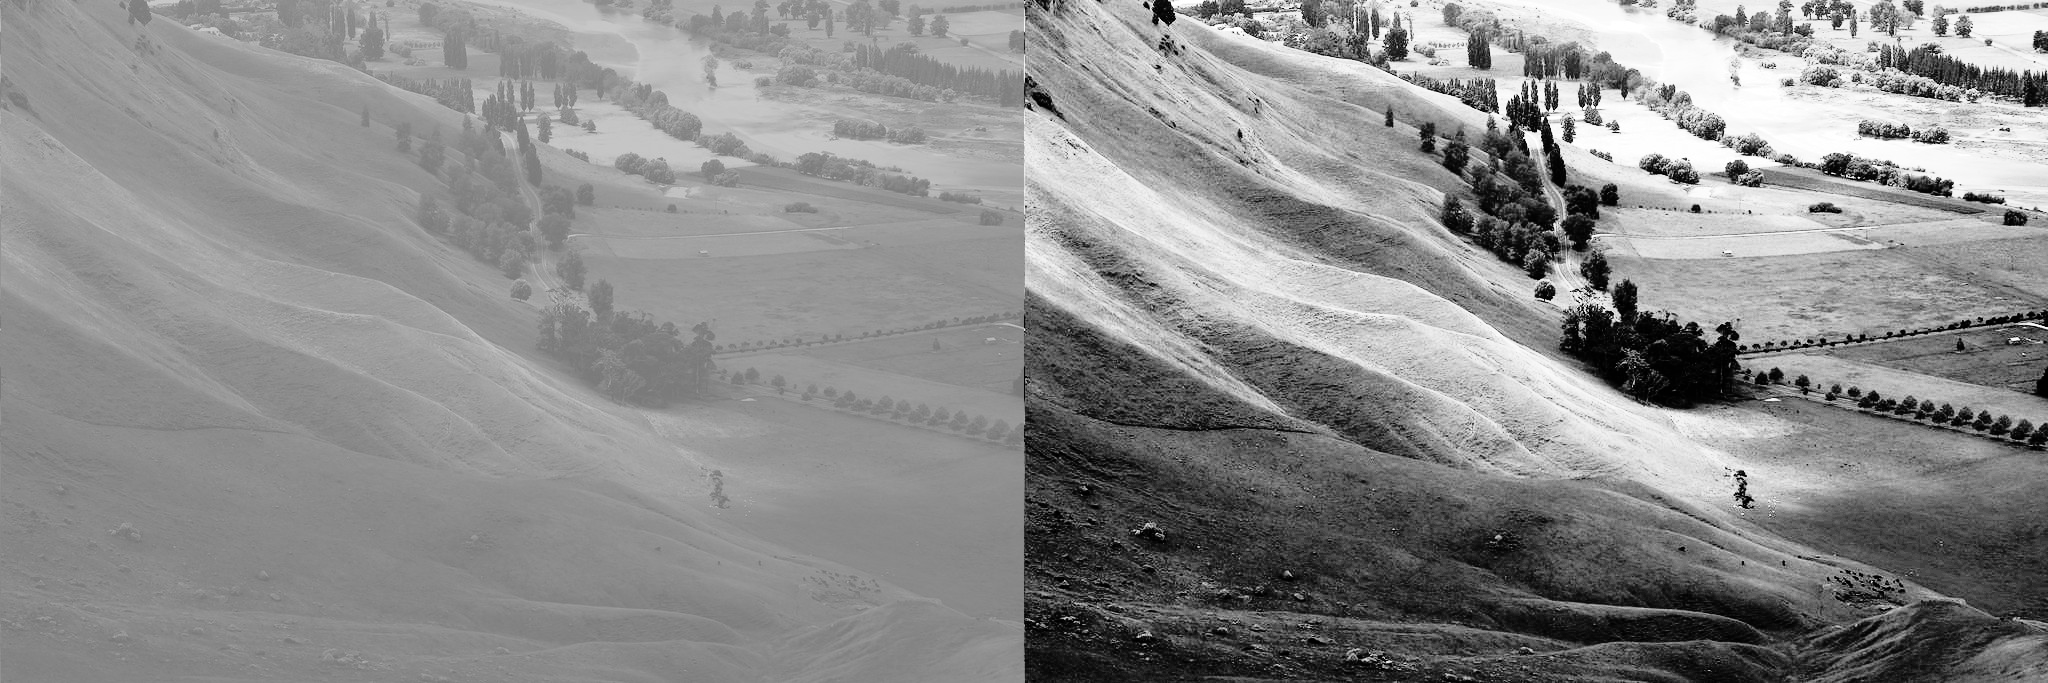
\includegraphics{ress.png} 이제 조명 조건이 다른 여러 이미지를 가져 와서
균등하게하고 결과를 확인할 수 있습니다.

히스토그램 등화는 이미지의 히스토그램이 특정 영역에 국한되어있을 때
유용합니다. 히스토그램이 넓은 영역을 포함하는 경우 (즉 밝은 픽셀과
어두운 픽셀이 모두있는 경우) 강도가 큰 곳에서는 잘 작동하지 않습니다.
추가 자료에서 SOF 링크를 확인하십시오.

\hypertarget{clahe-uxcf58uxd2b8uxb77cuxc2a4uxd2b8-uxc81cuxd55c-uxc801uxc751-uxd788uxc2a4uxd1a0uxadf8uxb7a8-uxc774uxd004uxb77cuxc774uxc81cuxc774uxc158r}{%
\subparagraph{CLAHE (콘트라스트 제한 적응 히스토그램
이퀄라이제이션)r}\label{clahe-uxcf58uxd2b8uxb77cuxc2a4uxd2b8-uxc81cuxd55c-uxc801uxc751-uxd788uxc2a4uxd1a0uxadf8uxb7a8-uxc774uxd004uxb77cuxc774uxc81cuxc774uxc158r}}

우리가 방금 본 첫 번째 히스토그램 평준화는 이미지의 전체 대비를
고려합니다. 많은 경우에, 그것은 좋은 생각이 아닙니다. 예를 들어 아래
이미지는 글로벌 히스토그램 균등화 후의 입력 이미지와 결과를 보여줍니다.

    \begin{Verbatim}[commandchars=\\\{\}]
{\color{incolor}In [{\color{incolor}32}]:} \PY{k+kn}{import} \PY{n+nn}{cv2} \PY{k}{as} \PY{n+nn}{cv}
         \PY{k+kn}{import} \PY{n+nn}{numpy} \PY{k}{as} \PY{n+nn}{np}
         \PY{k+kn}{import} \PY{n+nn}{bonghanUtil} \PY{k}{as} \PY{n+nn}{util}
         \PY{k+kn}{from} \PY{n+nn}{matplotlib} \PY{k}{import} \PY{n}{pyplot} \PY{k}{as} \PY{n}{plt}
         
         \PY{n}{img} \PY{o}{=} \PY{n}{cv}\PY{o}{.}\PY{n}{imread}\PY{p}{(}\PY{l+s+s1}{\PYZsq{}}\PY{l+s+s1}{clahe.png}\PY{l+s+s1}{\PYZsq{}}\PY{p}{,} \PY{l+m+mi}{0}\PY{p}{)}
         \PY{n}{equ} \PY{o}{=} \PY{n}{cv}\PY{o}{.}\PY{n}{equalizeHist}\PY{p}{(}\PY{n}{img}\PY{p}{)}
         \PY{n}{res} \PY{o}{=} \PY{n}{np}\PY{o}{.}\PY{n}{hstack}\PY{p}{(}\PY{p}{(}\PY{n}{img}\PY{p}{,} \PY{n}{equ}\PY{p}{)}\PY{p}{)} \PY{c+c1}{\PYZsh{}stacking images side\PYZhy{}by\PYZhy{}side}
         
         \PY{n}{plt}\PY{o}{.}\PY{n}{imshow}\PY{p}{(}\PY{n}{res}\PY{p}{,} \PY{n}{cmap} \PY{o}{=} \PY{l+s+s1}{\PYZsq{}}\PY{l+s+s1}{gray}\PY{l+s+s1}{\PYZsq{}}\PY{p}{)}
         \PY{n}{plt}\PY{o}{.}\PY{n}{show}\PY{p}{(}\PY{p}{)}
\end{Verbatim}


    \begin{center}
    \adjustimage{max size={0.9\linewidth}{0.9\paperheight}}{output_18_0.png}
    \end{center}
    { \hspace*{\fill} \\}
    
    히스토그램 평준화 후에 배경 대비가 향상되었습니다. 그러나 두 이미지에서
동상의 얼굴을 비교하십시오. 우리는 과도한 밝기로 인해 대부분의 정보를
잃어 버렸습니다. 이전의 경우에서 보았 듯이 히스토그램이 특정 영역에만
국한되어 있지 않기 때문입니다 (입력 이미지의 히스토그램을 그리면 더
직관적으로됩니다).

따라서이 문제를 해결하기 위해 \textbf{적응형 히스토그램 등화} 가
사용됩니다. 이 이미지는 \textbf{``타일''이라고 불리는 작은 블록으로
나뉩니다 (tileCount는 OpenCV에서 기본적으로 8x8입니다)}. 그런 다음 각
\textbf{블록은 평소처럼 히스토그램 평준화}됩니다. 따라서 작은 영역에서는
히스토그램이 작은 영역으로 한정됩니다 (노이즈가있는 경우 제외). 소음이
있으면 증폭 될 것입니다. 이를 방지하기 위해 \textbf{대비 제한 이
적용}됩니다. 히스토그램 빈이 지정된 명암 대비 한도 (기본적으로
OpenCV에서 40)보다 높으면 \textbf{히스토그램 평준화를 적용하기 전에 해당
픽셀을 다른 빈으로 균등하게 분배}합니다. 균등화 후, 타일 경계에서
\textbf{아티팩트를 제거하기 위해 쌍 선형 보간이 적용}됩니다.

Below code snippet shows how to apply CLAHE in OpenCV:

    \begin{Verbatim}[commandchars=\\\{\}]
{\color{incolor}In [{\color{incolor}33}]:} \PY{k+kn}{import} \PY{n+nn}{numpy} \PY{k}{as} \PY{n+nn}{np}
         \PY{k+kn}{import} \PY{n+nn}{cv2} \PY{k}{as} \PY{n+nn}{cv}
         \PY{k+kn}{from} \PY{n+nn}{matplotlib} \PY{k}{import} \PY{n}{pyplot} \PY{k}{as} \PY{n}{plt}
         
         \PY{n}{img} \PY{o}{=} \PY{n}{cv}\PY{o}{.}\PY{n}{imread}\PY{p}{(}\PY{l+s+s1}{\PYZsq{}}\PY{l+s+s1}{clahe.png}\PY{l+s+s1}{\PYZsq{}}\PY{p}{,} \PY{l+m+mi}{0}\PY{p}{)}
         
         \PY{c+c1}{\PYZsh{} create a CLAHE object (Arguments are optional).}
         \PY{n}{clahe} \PY{o}{=} \PY{n}{cv}\PY{o}{.}\PY{n}{createCLAHE}\PY{p}{(}\PY{n}{clipLimit} \PY{o}{=} \PY{l+m+mf}{2.0}\PY{p}{,} \PY{n}{tileGridSize} \PY{o}{=} \PY{p}{(}\PY{l+m+mi}{8}\PY{p}{,}\PY{l+m+mi}{8}\PY{p}{)}\PY{p}{)}
         \PY{n}{cl1}   \PY{o}{=} \PY{n}{clahe}\PY{o}{.}\PY{n}{apply}\PY{p}{(}\PY{n}{img}\PY{p}{)}
         \PY{n}{cv}\PY{o}{.}\PY{n}{imwrite}\PY{p}{(}\PY{l+s+s1}{\PYZsq{}}\PY{l+s+s1}{clahe\PYZus{}2.jpg}\PY{l+s+s1}{\PYZsq{}}\PY{p}{,} \PY{n}{cl1}\PY{p}{)}
         
         \PY{n}{res} \PY{o}{=} \PY{n}{np}\PY{o}{.}\PY{n}{hstack}\PY{p}{(}\PY{p}{(}\PY{n}{img}\PY{p}{,} \PY{n}{cl1}\PY{p}{)}\PY{p}{)}
         
         \PY{n}{plt}\PY{o}{.}\PY{n}{imshow}\PY{p}{(}\PY{n}{res}\PY{p}{,} \PY{n}{cmap} \PY{o}{=} \PY{l+s+s1}{\PYZsq{}}\PY{l+s+s1}{gray}\PY{l+s+s1}{\PYZsq{}}\PY{p}{)}
         \PY{n}{plt}\PY{o}{.}\PY{n}{show}\PY{p}{(}\PY{p}{)}
\end{Verbatim}


    \begin{center}
    \adjustimage{max size={0.9\linewidth}{0.9\paperheight}}{output_20_0.png}
    \end{center}
    { \hspace*{\fill} \\}
    
    Additional Resources

\begin{enumerate}
\def\labelenumi{\arabic{enumi}.}
\tightlist
\item
  Wikipedia page on
  \href{https://en.wikipedia.org/wiki/Histogram_equalization}{Histogram
  Equalization}
\item
  \href{https://docs.scipy.org/doc/numpy/reference/maskedarray.html}{Masked
  Arrays in Numpy}
\end{enumerate}

Also check these SOF questions regarding contrast adjustment:

\begin{enumerate}
\def\labelenumi{\arabic{enumi}.}
\setcounter{enumi}{2}
\tightlist
\item
  \href{https://stackoverflow.com/questions/10549245/how-can-i-adjust-contrast-in-opencv-in-c}{How
  can I adjust contrast in OpenCV in C?}
\item
  \href{https://stackoverflow.com/questions/10561222/how-do-i-equalize-contrast-brightness-of-images-using-opencv}{How
  do I equalize contrast \& brightness of images using opencv?}
\end{enumerate}

    \hypertarget{histograms---3-2d-histograms}{%
\paragraph{Histograms - 3 : 2D
Histograms}\label{histograms---3-2d-histograms}}

Learn to find and plot 2D Histograms

\hypertarget{uxbaa9uxd45c}{%
\subparagraph{목표}\label{uxbaa9uxd45c}}

In this chapter, we will learn to find and plot 2D histograms. It will
be helpful in coming chapters.

\hypertarget{introduction}{%
\subparagraph{Introduction}\label{introduction}}

첫 번째 기사에서는 1 차원 히스토그램을 계산하고 플롯했습니다. 우리는 한
가지 특징, 즉 픽셀의 그레이 스케일 강도 값을 고려하기 때문에 1
차원이라고합니다. 그러나 2 차원 히스토그램에서 두 가지 기능을
고려해야합니다. 일반적으로 두 개의 피쳐가 모든 픽셀의 색조 및 채도 값인
색상 히스토그램을 찾는 데 사용됩니다.

색상 히스토그램을 찾기위한 python 샘플 (samples / python /
color\_histogram.py)이 이미 있습니다. 우리는 그러한 색상 히스토그램을
만드는 방법을 이해하려고 노력할 것이며 히스토그램 백 프로젝션과 같은
추가 주제를 이해하는 데 유용 할 것입니다.

\hypertarget{d-histogram-in-opencv}{%
\subparagraph{2D Histogram in OpenCV}\label{d-histogram-in-opencv}}

이것은 매우 단순하며 동일한 함수 cv.calcHist ()를 사용하여 계산됩니다 .
색상 히스토그램의 경우 이미지를 BGR에서 HSV로 변환해야합니다. (1D
히스토그램의 경우 BGR에서 Grayscale로 변환됨을 기억하십시오.) 2D
히스토그램의 경우 매개 변수가 다음과 같이 수정됩니다.

\begin{itemize}
\tightlist
\item
  channels = {[}0,1{]} 왜냐하면 우리는 H와 S 평면을 모두 처리해야하기
  때문입니다.
\item
  bins = {[}180,256{]} H 평면의 경우 180, S 평면의 경우 256.
\item
  범위 = {[}0,180,0,256{]} 색조 값은 0과 180 사이에 있고 채도는 0과 256
  사이에 있습니다.
\end{itemize}

Now check the code below:

    \begin{Verbatim}[commandchars=\\\{\}]
{\color{incolor}In [{\color{incolor}24}]:} \PY{k+kn}{import} \PY{n+nn}{numpy} \PY{k}{as} \PY{n+nn}{np}
         \PY{k+kn}{import} \PY{n+nn}{cv2} \PY{k}{as} \PY{n+nn}{cv}
         \PY{k+kn}{from} \PY{n+nn}{matplotlib} \PY{k}{import} \PY{n}{pyplot} \PY{k}{as} \PY{n}{plt}
         
         \PY{n}{img} \PY{o}{=} \PY{n}{cv}\PY{o}{.}\PY{n}{imread}\PY{p}{(}\PY{l+s+s1}{\PYZsq{}}\PY{l+s+s1}{home4.jpg}\PY{l+s+s1}{\PYZsq{}}\PY{p}{)}
         
         \PY{n}{hsv} \PY{o}{=} \PY{n}{cv}\PY{o}{.}\PY{n}{cvtColor}\PY{p}{(}\PY{n}{img}\PY{p}{,}\PY{n}{cv}\PY{o}{.}\PY{n}{COLOR\PYZus{}BGR2HSV}\PY{p}{)}
         \PY{n}{hist} \PY{o}{=} \PY{n}{cv}\PY{o}{.}\PY{n}{calcHist}\PY{p}{(}\PY{p}{[}\PY{n}{hsv}\PY{p}{]}\PY{p}{,} \PY{p}{[}\PY{l+m+mi}{0}\PY{p}{,} \PY{l+m+mi}{1}\PY{p}{]}\PY{p}{,} \PY{k+kc}{None}\PY{p}{,} \PY{p}{[}\PY{l+m+mi}{180}\PY{p}{,} \PY{l+m+mi}{256}\PY{p}{]}\PY{p}{,} \PY{p}{[}\PY{l+m+mi}{0}\PY{p}{,} \PY{l+m+mi}{180}\PY{p}{,} \PY{l+m+mi}{0}\PY{p}{,} \PY{l+m+mi}{256}\PY{p}{]}\PY{p}{)}
         
         \PY{n}{plt}\PY{o}{.}\PY{n}{imshow}\PY{p}{(}\PY{n}{hist}\PY{p}{,} \PY{n}{interpolation} \PY{o}{=} \PY{l+s+s1}{\PYZsq{}}\PY{l+s+s1}{nearest}\PY{l+s+s1}{\PYZsq{}} \PY{p}{)}
         \PY{n}{plt}\PY{o}{.}\PY{n}{show}\PY{p}{(}\PY{p}{)}
\end{Verbatim}


    \begin{center}
    \adjustimage{max size={0.9\linewidth}{0.9\paperheight}}{output_23_0.png}
    \end{center}
    { \hspace*{\fill} \\}
    
    \hypertarget{d-histogram-in-numpy}{%
\paragraph{2D Histogram in Numpy}\label{d-histogram-in-numpy}}

Numpy also provides a specific function for this : np.histogram2d().
(Remember, for 1D histogram we used np.histogram() ).

    \begin{Verbatim}[commandchars=\\\{\}]
{\color{incolor}In [{\color{incolor}52}]:} \PY{k+kn}{import} \PY{n+nn}{numpy} \PY{k}{as} \PY{n+nn}{np}
         \PY{k+kn}{import} \PY{n+nn}{cv2} \PY{k}{as} \PY{n+nn}{cv}
         \PY{k+kn}{from} \PY{n+nn}{matplotlib} \PY{k}{import} \PY{n}{pyplot} \PY{k}{as} \PY{n}{plt}
         
         \PY{n}{img} \PY{o}{=} \PY{n}{cv}\PY{o}{.}\PY{n}{imread}\PY{p}{(}\PY{l+s+s1}{\PYZsq{}}\PY{l+s+s1}{home4.jpg}\PY{l+s+s1}{\PYZsq{}}\PY{p}{)}
         
         \PY{n}{hsv\PYZus{}map} \PY{o}{=} \PY{n}{np}\PY{o}{.}\PY{n}{zeros}\PY{p}{(}\PY{p}{(}\PY{l+m+mi}{180}\PY{p}{,} \PY{l+m+mi}{256}\PY{p}{,} \PY{l+m+mi}{3}\PY{p}{)}\PY{p}{,} \PY{n}{np}\PY{o}{.}\PY{n}{uint8}\PY{p}{)}
         \PY{n}{h}\PY{p}{,} \PY{n}{s} \PY{o}{=} \PY{n}{np}\PY{o}{.}\PY{n}{indices}\PY{p}{(}\PY{n}{hsv\PYZus{}map}\PY{o}{.}\PY{n}{shape}\PY{p}{[}\PY{p}{:}\PY{l+m+mi}{2}\PY{p}{]}\PY{p}{)}
         \PY{n}{hsv\PYZus{}map}\PY{p}{[}\PY{p}{:}\PY{p}{,}\PY{p}{:}\PY{p}{,}\PY{l+m+mi}{0}\PY{p}{]} \PY{o}{=} \PY{n}{h}
         \PY{n}{hsv\PYZus{}map}\PY{p}{[}\PY{p}{:}\PY{p}{,}\PY{p}{:}\PY{p}{,}\PY{l+m+mi}{1}\PY{p}{]} \PY{o}{=} \PY{n}{s}
         \PY{n}{hsv\PYZus{}map}\PY{p}{[}\PY{p}{:}\PY{p}{,}\PY{p}{:}\PY{p}{,}\PY{l+m+mi}{2}\PY{p}{]} \PY{o}{=} \PY{l+m+mi}{255}
         \PY{n}{hsv\PYZus{}map} \PY{o}{=} \PY{n}{cv}\PY{o}{.}\PY{n}{cvtColor}\PY{p}{(}\PY{n}{hsv\PYZus{}map}\PY{p}{,} \PY{n}{cv}\PY{o}{.}\PY{n}{COLOR\PYZus{}HSV2BGR}\PY{p}{)}
         
         \PY{n}{hsv} \PY{o}{=} \PY{n}{cv}\PY{o}{.}\PY{n}{cvtColor}\PY{p}{(}\PY{n}{img}\PY{p}{,} \PY{n}{cv}\PY{o}{.}\PY{n}{COLOR\PYZus{}BGR2HSV}\PY{p}{)}
         \PY{n}{h}\PY{p}{,} \PY{n}{s}\PY{p}{,} \PY{n}{\PYZus{}} \PY{o}{=} \PY{n}{cv}\PY{o}{.}\PY{n}{split}\PY{p}{(}\PY{n}{hsv}\PY{p}{)}
         \PY{n}{hist}\PY{p}{,} \PY{n}{xbins}\PY{p}{,} \PY{n}{ybins} \PY{o}{=} \PY{n}{np}\PY{o}{.}\PY{n}{histogram2d}\PY{p}{(}\PY{n}{h}\PY{o}{.}\PY{n}{ravel}\PY{p}{(}\PY{p}{)}\PY{p}{,}\PY{n}{s}\PY{o}{.}\PY{n}{ravel}\PY{p}{(}\PY{p}{)}\PY{p}{,}\PY{p}{[}\PY{l+m+mi}{180}\PY{p}{,}\PY{l+m+mi}{256}\PY{p}{]}\PY{p}{,}\PY{p}{[}\PY{p}{[}\PY{l+m+mi}{0}\PY{p}{,}\PY{l+m+mi}{180}\PY{p}{]}\PY{p}{,}\PY{p}{[}\PY{l+m+mi}{0}\PY{p}{,}\PY{l+m+mi}{256}\PY{p}{]}\PY{p}{]}\PY{p}{)}
         
         \PY{n}{plt}\PY{o}{.}\PY{n}{imshow}\PY{p}{(}\PY{n}{hist}\PY{p}{,} \PY{n}{interpolation} \PY{o}{=} \PY{l+s+s1}{\PYZsq{}}\PY{l+s+s1}{nearest}\PY{l+s+s1}{\PYZsq{}} \PY{p}{)}
         \PY{n}{plt}\PY{o}{.}\PY{n}{show}\PY{p}{(}\PY{p}{)}
\end{Verbatim}


    \begin{center}
    \adjustimage{max size={0.9\linewidth}{0.9\paperheight}}{output_25_0.png}
    \end{center}
    { \hspace*{\fill} \\}
    
    \begin{Verbatim}[commandchars=\\\{\}]
{\color{incolor}In [{\color{incolor}26}]:} \PY{k+kn}{import} \PY{n+nn}{numpy} \PY{k}{as} \PY{n+nn}{np}
         \PY{k+kn}{import} \PY{n+nn}{cv2} \PY{k}{as} \PY{n+nn}{cv}
         
         
         \PY{n}{hsv\PYZus{}map} \PY{o}{=} \PY{n}{np}\PY{o}{.}\PY{n}{zeros}\PY{p}{(}\PY{p}{(}\PY{l+m+mi}{180}\PY{p}{,} \PY{l+m+mi}{256}\PY{p}{,} \PY{l+m+mi}{3}\PY{p}{)}\PY{p}{,} \PY{n}{np}\PY{o}{.}\PY{n}{uint8}\PY{p}{)}
         \PY{n}{h}\PY{p}{,} \PY{n}{s} \PY{o}{=} \PY{n}{np}\PY{o}{.}\PY{n}{indices}\PY{p}{(}\PY{n}{hsv\PYZus{}map}\PY{o}{.}\PY{n}{shape}\PY{p}{[}\PY{p}{:}\PY{l+m+mi}{2}\PY{p}{]}\PY{p}{)}
         \PY{n}{hsv\PYZus{}map}\PY{p}{[}\PY{p}{:}\PY{p}{,}\PY{p}{:}\PY{p}{,}\PY{l+m+mi}{0}\PY{p}{]} \PY{o}{=} \PY{n}{h}
         \PY{n}{hsv\PYZus{}map}\PY{p}{[}\PY{p}{:}\PY{p}{,}\PY{p}{:}\PY{p}{,}\PY{l+m+mi}{1}\PY{p}{]} \PY{o}{=} \PY{n}{s}
         \PY{n}{hsv\PYZus{}map}\PY{p}{[}\PY{p}{:}\PY{p}{,}\PY{p}{:}\PY{p}{,}\PY{l+m+mi}{2}\PY{p}{]} \PY{o}{=} \PY{l+m+mi}{255}
         \PY{n}{hsv\PYZus{}map} \PY{o}{=} \PY{n}{cv}\PY{o}{.}\PY{n}{cvtColor}\PY{p}{(}\PY{n}{hsv\PYZus{}map}\PY{p}{,} \PY{n}{cv}\PY{o}{.}\PY{n}{COLOR\PYZus{}HSV2BGR}\PY{p}{)}
         \PY{n}{cv}\PY{o}{.}\PY{n}{imshow}\PY{p}{(}\PY{l+s+s1}{\PYZsq{}}\PY{l+s+s1}{hsv\PYZus{}map}\PY{l+s+s1}{\PYZsq{}}\PY{p}{,} \PY{n}{hsv\PYZus{}map}\PY{p}{)}
         
         \PY{n}{cv}\PY{o}{.}\PY{n}{namedWindow}\PY{p}{(}\PY{l+s+s1}{\PYZsq{}}\PY{l+s+s1}{hist}\PY{l+s+s1}{\PYZsq{}}\PY{p}{,} \PY{l+m+mi}{0}\PY{p}{)}
         \PY{n}{hist\PYZus{}scale} \PY{o}{=} \PY{l+m+mi}{10}
         
         \PY{k}{def} \PY{n+nf}{set\PYZus{}scale}\PY{p}{(}\PY{n}{val}\PY{p}{)}\PY{p}{:}
             \PY{k}{global} \PY{n}{hist\PYZus{}scale}
             \PY{n}{hist\PYZus{}scale} \PY{o}{=} \PY{n}{val}
         \PY{n}{cv}\PY{o}{.}\PY{n}{createTrackbar}\PY{p}{(}\PY{l+s+s1}{\PYZsq{}}\PY{l+s+s1}{scale}\PY{l+s+s1}{\PYZsq{}}\PY{p}{,} \PY{l+s+s1}{\PYZsq{}}\PY{l+s+s1}{hist}\PY{l+s+s1}{\PYZsq{}}\PY{p}{,} \PY{n}{hist\PYZus{}scale}\PY{p}{,} \PY{l+m+mi}{32}\PY{p}{,} \PY{n}{set\PYZus{}scale}\PY{p}{)}
         
         \PY{k}{try}\PY{p}{:}
             \PY{n}{fn} \PY{o}{=} \PY{n}{sys}\PY{o}{.}\PY{n}{argv}\PY{p}{[}\PY{l+m+mi}{1}\PY{p}{]}
         \PY{k}{except}\PY{p}{:}
             \PY{n}{fn} \PY{o}{=} \PY{l+m+mi}{0}
         
         \PY{n}{frame} \PY{o}{=} \PY{n}{cv}\PY{o}{.}\PY{n}{imread}\PY{p}{(}\PY{l+s+s1}{\PYZsq{}}\PY{l+s+s1}{home4.jpg}\PY{l+s+s1}{\PYZsq{}}\PY{p}{)}
         
         \PY{k}{while} \PY{k+kc}{True}\PY{p}{:}
             \PY{n}{cv}\PY{o}{.}\PY{n}{imshow}\PY{p}{(}\PY{l+s+s1}{\PYZsq{}}\PY{l+s+s1}{camera}\PY{l+s+s1}{\PYZsq{}}\PY{p}{,} \PY{n}{frame}\PY{p}{)}
         
             \PY{n}{small} \PY{o}{=} \PY{n}{cv}\PY{o}{.}\PY{n}{pyrDown}\PY{p}{(}\PY{n}{frame}\PY{p}{)}
         
             \PY{n}{hsv} \PY{o}{=} \PY{n}{cv}\PY{o}{.}\PY{n}{cvtColor}\PY{p}{(}\PY{n}{small}\PY{p}{,} \PY{n}{cv}\PY{o}{.}\PY{n}{COLOR\PYZus{}BGR2HSV}\PY{p}{)}
             \PY{n}{dark} \PY{o}{=} \PY{n}{hsv}\PY{p}{[}\PY{o}{.}\PY{o}{.}\PY{o}{.}\PY{p}{,}\PY{l+m+mi}{2}\PY{p}{]} \PY{o}{\PYZlt{}} \PY{l+m+mi}{32}
             \PY{n}{hsv}\PY{p}{[}\PY{n}{dark}\PY{p}{]} \PY{o}{=} \PY{l+m+mi}{0}
             \PY{n}{h} \PY{o}{=} \PY{n}{cv}\PY{o}{.}\PY{n}{calcHist}\PY{p}{(}\PY{p}{[}\PY{n}{hsv}\PY{p}{]}\PY{p}{,} \PY{p}{[}\PY{l+m+mi}{0}\PY{p}{,} \PY{l+m+mi}{1}\PY{p}{]}\PY{p}{,} \PY{k+kc}{None}\PY{p}{,} \PY{p}{[}\PY{l+m+mi}{180}\PY{p}{,} \PY{l+m+mi}{256}\PY{p}{]}\PY{p}{,} \PY{p}{[}\PY{l+m+mi}{0}\PY{p}{,} \PY{l+m+mi}{180}\PY{p}{,} \PY{l+m+mi}{0}\PY{p}{,} \PY{l+m+mi}{256}\PY{p}{]}\PY{p}{)}
         
             \PY{n}{h} \PY{o}{=} \PY{n}{np}\PY{o}{.}\PY{n}{clip}\PY{p}{(}\PY{n}{h}\PY{o}{*}\PY{l+m+mf}{0.005}\PY{o}{*}\PY{n}{hist\PYZus{}scale}\PY{p}{,} \PY{l+m+mi}{0}\PY{p}{,} \PY{l+m+mi}{1}\PY{p}{)}
             \PY{n}{vis} \PY{o}{=} \PY{n}{hsv\PYZus{}map}\PY{o}{*}\PY{n}{h}\PY{p}{[}\PY{p}{:}\PY{p}{,}\PY{p}{:}\PY{p}{,}\PY{n}{np}\PY{o}{.}\PY{n}{newaxis}\PY{p}{]} \PY{o}{/} \PY{l+m+mf}{255.0}
             \PY{n}{cv}\PY{o}{.}\PY{n}{imshow}\PY{p}{(}\PY{l+s+s1}{\PYZsq{}}\PY{l+s+s1}{hist}\PY{l+s+s1}{\PYZsq{}}\PY{p}{,} \PY{n}{vis}\PY{p}{)}
         
             \PY{n}{ch} \PY{o}{=} \PY{n}{cv}\PY{o}{.}\PY{n}{waitKey}\PY{p}{(}\PY{l+m+mi}{1}\PY{p}{)}
             \PY{k}{if} \PY{n}{ch} \PY{o}{==} \PY{l+m+mi}{27}\PY{p}{:}
                 \PY{k}{break}
                 
         \PY{n}{cv}\PY{o}{.}\PY{n}{destroyAllWindows}\PY{p}{(}\PY{p}{)}
\end{Verbatim}


    \hypertarget{histogram---4-histogram-backprojection}{%
\paragraph{Histogram - 4 : Histogram
Backprojection}\label{histogram---4-histogram-backprojection}}

Learn histogram backprojection to segment colored objects

\hypertarget{uxbaa9uxd45c}{%
\subparagraph{목표}\label{uxbaa9uxd45c}}

In this chapter, we will learn about histogram backprojection.

\hypertarget{uxc774uxb860}{%
\subparagraph{이론}\label{uxc774uxb860}}

마이클 J. 스와 인 (Michael J. Swain), 데이나 H. 발라드 (Dana H. Ballard)
가 자신의 논문 에서 색 막대 그래프를 통한 인덱싱을 제안했습니다 .

실제로 간단한 단어로 무엇입니까? 이미지 세분화 또는 이미지에서 관심있는
대상을 찾는 데 사용됩니다. 간단히 말하면 입력 이미지와 동일한 크기 (단
채널)의 이미지를 만듭니다. 각 픽셀은 해당 픽셀이 우리 객체에 속할 확률에
해당합니다. 보다 단순한 세계에서, 출력 이미지는 남은 부분에 비해 더 많은
흰색의 관심 대상을 갖게됩니다. 음, 직관적 인 설명입니다. (나는 그것을 더
간단하게 만들 수 없다). 히스토그램 Backprojection은 캠 쉬프트 알고리즘
등에서 사용됩니다.

어떻게해야합니까? 우리는 우리의 관심 대상 (우리의 경우, 땅, 플레이어 및
다른 것들을 남겨둔 채)을 포함하는 이미지의 히스토그램을 생성합니다. 더
나은 결과를 얻으려면 개체가 가능한 한 이미지를 채워야합니다. 그리고
그레이 스케일 히스토그램보다 컬러 히스토그램이 더 좋습니다. 왜냐하면
오브젝트의 색상이 그레이 스케일 강도보다 오브젝트를 정의하는 더 좋은
방법이기 때문입니다. 그런 다음 우리가 객체를 찾을 필요가있는 테스트
이미지 위에이 히스토그램을 ``백 - 프로젝트''합니다. 다시 말하면, 우리는
땅에 속한 모든 픽셀의 확률을 계산하여 보여줍니다. 적절한 thresholding에
대한 결과 출력은 우리에게 하나의 근거만을 제공합니다.

\hypertarget{numpyuxc758-uxc54cuxace0uxb9acuxc998}{%
\subparagraph{Numpy의
알고리즘}\label{numpyuxc758-uxc54cuxace0uxb9acuxc998}}

\begin{enumerate}
\def\labelenumi{\arabic{enumi}.}
\tightlist
\item
  먼저 우리가 찾을 필요가있는 대상 ( `M')과 검색 할 대상 (
  'I'이되도록)의 색상 히스토그램을 계산해야합니다.
\end{enumerate}

    \begin{Verbatim}[commandchars=\\\{\}]
{\color{incolor}In [{\color{incolor}1}]:} \PY{k+kn}{import} \PY{n+nn}{numpy} \PY{k}{as} \PY{n+nn}{np}
        \PY{k+kn}{import} \PY{n+nn}{cv2} \PY{k}{as} \PY{n+nn}{cv}
        \PY{k+kn}{from} \PY{n+nn}{matplotlib} \PY{k}{import} \PY{n}{pyplot} \PY{k}{as} \PY{n}{plt}
        \PY{k+kn}{import} \PY{n+nn}{bonghanUtil} \PY{k}{as} \PY{n+nn}{util}
        
        \PY{c+c1}{\PYZsh{}roi is the object or region of object we need to find}
        \PY{n}{roi} \PY{o}{=} \PY{n}{cv}\PY{o}{.}\PY{n}{imread}\PY{p}{(}\PY{l+s+s1}{\PYZsq{}}\PY{l+s+s1}{fruit\PYZus{}piece.jpg}\PY{l+s+s1}{\PYZsq{}}\PY{p}{)}
        \PY{n}{hsv} \PY{o}{=} \PY{n}{cv}\PY{o}{.}\PY{n}{cvtColor}\PY{p}{(}\PY{n}{roi}\PY{p}{,} \PY{n}{cv}\PY{o}{.}\PY{n}{COLOR\PYZus{}BGR2HSV}\PY{p}{)}
        
        \PY{c+c1}{\PYZsh{}target is the image we search in}
        \PY{n}{target} \PY{o}{=} \PY{n}{cv}\PY{o}{.}\PY{n}{imread}\PY{p}{(}\PY{l+s+s1}{\PYZsq{}}\PY{l+s+s1}{fruit.jpg}\PY{l+s+s1}{\PYZsq{}}\PY{p}{)}
        \PY{n}{hsvt}   \PY{o}{=} \PY{n}{cv}\PY{o}{.}\PY{n}{cvtColor}\PY{p}{(}\PY{n}{target}\PY{p}{,} \PY{n}{cv}\PY{o}{.}\PY{n}{COLOR\PYZus{}BGR2HSV}\PY{p}{)}
        
        \PY{c+c1}{\PYZsh{} Find the histograms using calcHist. Can be done with np.histogram2d also}
        \PY{n}{M} \PY{o}{=} \PY{n}{cv}\PY{o}{.}\PY{n}{calcHist}\PY{p}{(}\PY{p}{[}\PY{n}{hsv}\PY{p}{]} \PY{p}{,}\PY{p}{[}\PY{l+m+mi}{0}\PY{p}{,} \PY{l+m+mi}{1}\PY{p}{]}\PY{p}{,} \PY{k+kc}{None}\PY{p}{,} \PY{p}{[}\PY{l+m+mi}{180}\PY{p}{,} \PY{l+m+mi}{256}\PY{p}{]}\PY{p}{,} \PY{p}{[}\PY{l+m+mi}{0}\PY{p}{,} \PY{l+m+mi}{180}\PY{p}{,} \PY{l+m+mi}{0}\PY{p}{,} \PY{l+m+mi}{256}\PY{p}{]} \PY{p}{)}
        \PY{n}{I} \PY{o}{=} \PY{n}{cv}\PY{o}{.}\PY{n}{calcHist}\PY{p}{(}\PY{p}{[}\PY{n}{hsvt}\PY{p}{]}\PY{p}{,}\PY{p}{[}\PY{l+m+mi}{0}\PY{p}{,} \PY{l+m+mi}{1}\PY{p}{]}\PY{p}{,} \PY{k+kc}{None}\PY{p}{,} \PY{p}{[}\PY{l+m+mi}{180}\PY{p}{,} \PY{l+m+mi}{256}\PY{p}{]}\PY{p}{,} \PY{p}{[}\PY{l+m+mi}{0}\PY{p}{,} \PY{l+m+mi}{180}\PY{p}{,} \PY{l+m+mi}{0}\PY{p}{,} \PY{l+m+mi}{256}\PY{p}{]} \PY{p}{)}
\end{Verbatim}


    \begin{enumerate}
\def\labelenumi{\arabic{enumi}.}
\setcounter{enumi}{1}
\tightlist
\item
  Find the ratio \(R=\frac{M}{I}\). Then backproject R, ie use R as
  palette and create a new image with every pixel as its corresponding
  probability of being target. ie B(x,y) = R{[}h(x,y),s(x,y){]} where h
  is hue and s is saturation of the pixel at (x,y). After that apply the
  condition \(B(x,y)=min[B(x,y),1]\).
\end{enumerate}

    \begin{Verbatim}[commandchars=\\\{\}]
{\color{incolor}In [{\color{incolor}3}]:} \PY{n}{h}\PY{p}{,}\PY{n}{s}\PY{p}{,}\PY{n}{\PYZus{}} \PY{o}{=} \PY{n}{cv}\PY{o}{.}\PY{n}{split}\PY{p}{(}\PY{n}{hsvt}\PY{p}{)}
        \PY{n}{R} \PY{o}{=} \PY{n}{M} \PY{o}{/} \PY{n}{I}
        \PY{n}{B}     \PY{o}{=} \PY{n}{R}\PY{p}{[}\PY{n}{h}\PY{o}{.}\PY{n}{ravel}\PY{p}{(}\PY{p}{)}\PY{p}{,} \PY{n}{s}\PY{o}{.}\PY{n}{ravel}\PY{p}{(}\PY{p}{)}\PY{p}{]}
        \PY{n}{B}     \PY{o}{=} \PY{n}{np}\PY{o}{.}\PY{n}{minimum}\PY{p}{(}\PY{n}{B}\PY{p}{,} \PY{l+m+mi}{1}\PY{p}{)}
        \PY{n}{B}     \PY{o}{=} \PY{n}{B}\PY{o}{.}\PY{n}{reshape}\PY{p}{(}\PY{n}{hsvt}\PY{o}{.}\PY{n}{shape}\PY{p}{[}\PY{p}{:}\PY{l+m+mi}{2}\PY{p}{]}\PY{p}{)}
\end{Verbatim}


    \begin{Verbatim}[commandchars=\\\{\}]
C:\textbackslash{}Users\textbackslash{}bongh\textbackslash{}Anaconda3\textbackslash{}envs\textbackslash{}p36\textbackslash{}lib\textbackslash{}site-packages\textbackslash{}ipykernel\_launcher.py:2: RuntimeWarning: invalid value encountered in true\_divide
  

    \end{Verbatim}

    \begin{enumerate}
\def\labelenumi{\arabic{enumi}.}
\setcounter{enumi}{2}
\tightlist
\item
  Now apply a convolution with a circular disc, B=D∗B, where D is the
  disc kernel.
\end{enumerate}

    \begin{Verbatim}[commandchars=\\\{\}]
{\color{incolor}In [{\color{incolor}4}]:} \PY{n}{disc} \PY{o}{=} \PY{n}{cv}\PY{o}{.}\PY{n}{getStructuringElement}\PY{p}{(}\PY{n}{cv}\PY{o}{.}\PY{n}{MORPH\PYZus{}ELLIPSE}\PY{p}{,} \PY{p}{(}\PY{l+m+mi}{5}\PY{p}{,} \PY{l+m+mi}{5}\PY{p}{)}\PY{p}{)}
        \PY{n}{cv}\PY{o}{.}\PY{n}{filter2D}\PY{p}{(}\PY{n}{B}\PY{p}{,} \PY{o}{\PYZhy{}}\PY{l+m+mi}{1}\PY{p}{,} \PY{n}{disc}\PY{p}{,} \PY{n}{B}\PY{p}{)}
        \PY{n}{B} \PY{o}{=} \PY{n}{np}\PY{o}{.}\PY{n}{uint8}\PY{p}{(}\PY{n}{B}\PY{p}{)}
        \PY{n}{cv}\PY{o}{.}\PY{n}{normalize}\PY{p}{(}\PY{n}{B}\PY{p}{,} \PY{n}{B}\PY{p}{,} \PY{l+m+mi}{0}\PY{p}{,} \PY{l+m+mi}{255}\PY{p}{,} \PY{n}{cv}\PY{o}{.}\PY{n}{NORM\PYZus{}MINMAX}\PY{p}{)}
\end{Verbatim}


\begin{Verbatim}[commandchars=\\\{\}]
{\color{outcolor}Out[{\color{outcolor}4}]:} array([[0, 0, 0, {\ldots}, 0, 0, 0],
               [0, 0, 0, {\ldots}, 0, 0, 0],
               [0, 0, 0, {\ldots}, 0, 0, 0],
               {\ldots},
               [0, 0, 0, {\ldots}, 0, 0, 0],
               [0, 0, 0, {\ldots}, 0, 0, 0],
               [0, 0, 0, {\ldots}, 0, 0, 0]], dtype=uint8)
\end{Verbatim}
            
    \begin{enumerate}
\def\labelenumi{\arabic{enumi}.}
\setcounter{enumi}{3}
\tightlist
\item
  Now the location of maximum intensity gives us the location of object.
  If we are expecting a region in the image, thresholding for a suitable
  value gives a nice result.
\end{enumerate}

    \begin{Verbatim}[commandchars=\\\{\}]
{\color{incolor}In [{\color{incolor}5}]:} \PY{n}{ret}\PY{p}{,}\PY{n}{thresh} \PY{o}{=} \PY{n}{cv}\PY{o}{.}\PY{n}{threshold}\PY{p}{(}\PY{n}{B}\PY{p}{,}\PY{l+m+mi}{50}\PY{p}{,}\PY{l+m+mi}{255}\PY{p}{,}\PY{l+m+mi}{0}\PY{p}{)}
        
        \PY{n}{util}\PY{o}{.}\PY{n}{showImage}\PY{p}{(}\PY{n}{thresh}\PY{p}{)}
\end{Verbatim}


    \hypertarget{backprojection-in-opencv}{%
\subparagraph{Backprojection in OpenCV}\label{backprojection-in-opencv}}

OpenCV는 inbuilt 함수 cv.calcBackProject ()를 제공합니다 . 그 매개
변수는 cv.calcHist () 함수 와 거의 같습니다 . 그 매개 변수 중 하나는
히스토그램입니다. 히스토그램은 객체의 히스토그램이며이를 찾아야합니다.
또한 객체 히스토그램은 backproject 함수에 전달되기 전에
정규화되어야합니다. 확률 이미지를 반환합니다. 그런 다음 이미지를 디스크
커널로 컨버그하고 임계 값을 적용합니다. 아래는 내 코드 및 출력입니다.

    \begin{Verbatim}[commandchars=\\\{\}]
{\color{incolor}In [{\color{incolor}9}]:} \PY{k+kn}{import} \PY{n+nn}{numpy} \PY{k}{as} \PY{n+nn}{np}
        \PY{k+kn}{import} \PY{n+nn}{cv2} \PY{k}{as} \PY{n+nn}{cv}
        
        \PY{n}{roi} \PY{o}{=} \PY{n}{cv}\PY{o}{.}\PY{n}{imread}\PY{p}{(}\PY{l+s+s1}{\PYZsq{}}\PY{l+s+s1}{fruit\PYZus{}piece.jpg}\PY{l+s+s1}{\PYZsq{}}\PY{p}{)}
        \PY{n}{hsv} \PY{o}{=} \PY{n}{cv}\PY{o}{.}\PY{n}{cvtColor}\PY{p}{(}\PY{n}{roi}\PY{p}{,} \PY{n}{cv}\PY{o}{.}\PY{n}{COLOR\PYZus{}BGR2HSV}\PY{p}{)}
        
        \PY{n}{target} \PY{o}{=} \PY{n}{cv}\PY{o}{.}\PY{n}{imread}\PY{p}{(}\PY{l+s+s1}{\PYZsq{}}\PY{l+s+s1}{fruit.jpg}\PY{l+s+s1}{\PYZsq{}}\PY{p}{)}
        \PY{n}{hsvt}   \PY{o}{=} \PY{n}{cv}\PY{o}{.}\PY{n}{cvtColor}\PY{p}{(}\PY{n}{target}\PY{p}{,} \PY{n}{cv}\PY{o}{.}\PY{n}{COLOR\PYZus{}BGR2HSV}\PY{p}{)}
        
        \PY{c+c1}{\PYZsh{} calculating object histogram}
        \PY{n}{roihist} \PY{o}{=} \PY{n}{cv}\PY{o}{.}\PY{n}{calcHist}\PY{p}{(}\PY{p}{[}\PY{n}{hsv}\PY{p}{]}\PY{p}{,}\PY{p}{[}\PY{l+m+mi}{0}\PY{p}{,} \PY{l+m+mi}{1}\PY{p}{]}\PY{p}{,} \PY{k+kc}{None}\PY{p}{,} \PY{p}{[}\PY{l+m+mi}{180}\PY{p}{,} \PY{l+m+mi}{256}\PY{p}{]}\PY{p}{,} \PY{p}{[}\PY{l+m+mi}{0}\PY{p}{,} \PY{l+m+mi}{180}\PY{p}{,} \PY{l+m+mi}{0}\PY{p}{,} \PY{l+m+mi}{256}\PY{p}{]} \PY{p}{)}
        
        \PY{c+c1}{\PYZsh{} normalize histogram and apply backprojection}
        \PY{n}{cv}\PY{o}{.}\PY{n}{normalize}\PY{p}{(}\PY{n}{roihist}\PY{p}{,} \PY{n}{roihist}\PY{p}{,} \PY{l+m+mi}{0}\PY{p}{,} \PY{l+m+mi}{255}\PY{p}{,} \PY{n}{cv}\PY{o}{.}\PY{n}{NORM\PYZus{}MINMAX}\PY{p}{)}
        \PY{n}{dst} \PY{o}{=} \PY{n}{cv}\PY{o}{.}\PY{n}{calcBackProject}\PY{p}{(}\PY{p}{[}\PY{n}{hsvt}\PY{p}{]}\PY{p}{,} \PY{p}{[}\PY{l+m+mi}{0}\PY{p}{,} \PY{l+m+mi}{1}\PY{p}{]}\PY{p}{,} \PY{n}{roihist}\PY{p}{,} \PY{p}{[}\PY{l+m+mi}{0}\PY{p}{,}\PY{l+m+mi}{180}\PY{p}{,}\PY{l+m+mi}{0}\PY{p}{,}\PY{l+m+mi}{256}\PY{p}{]}\PY{p}{,}\PY{l+m+mi}{1}\PY{p}{)}
        
        \PY{c+c1}{\PYZsh{} Now convolute with circular disc}
        \PY{n}{disc} \PY{o}{=} \PY{n}{cv}\PY{o}{.}\PY{n}{getStructuringElement}\PY{p}{(}\PY{n}{cv}\PY{o}{.}\PY{n}{MORPH\PYZus{}ELLIPSE}\PY{p}{,} \PY{p}{(}\PY{l+m+mi}{5}\PY{p}{,} \PY{l+m+mi}{5}\PY{p}{)}\PY{p}{)}
        \PY{n}{cv}\PY{o}{.}\PY{n}{filter2D}\PY{p}{(}\PY{n}{dst}\PY{p}{,} \PY{o}{\PYZhy{}}\PY{l+m+mi}{1}\PY{p}{,} \PY{n}{disc}\PY{p}{,} \PY{n}{dst}\PY{p}{)}
        
        \PY{c+c1}{\PYZsh{} threshold and binary AND}
        \PY{n}{ret}\PY{p}{,}\PY{n}{thresh} \PY{o}{=} \PY{n}{cv}\PY{o}{.}\PY{n}{threshold}\PY{p}{(}\PY{n}{dst}\PY{p}{,} \PY{l+m+mi}{50}\PY{p}{,} \PY{l+m+mi}{255}\PY{p}{,} \PY{l+m+mi}{0}\PY{p}{)}
        \PY{n}{thresh} \PY{o}{=} \PY{n}{cv}\PY{o}{.}\PY{n}{merge}\PY{p}{(}\PY{p}{(}\PY{n}{thresh}\PY{p}{,} \PY{n}{thresh}\PY{p}{,} \PY{n}{thresh}\PY{p}{)}\PY{p}{)}
        
        \PY{n}{res} \PY{o}{=} \PY{n}{cv}\PY{o}{.}\PY{n}{bitwise\PYZus{}and}\PY{p}{(}\PY{n}{target}\PY{p}{,}\PY{n}{thresh}\PY{p}{)}
        \PY{n}{res} \PY{o}{=} \PY{n}{np}\PY{o}{.}\PY{n}{vstack}\PY{p}{(}\PY{p}{(}\PY{n}{target}\PY{p}{,}\PY{n}{thresh}\PY{p}{,}\PY{n}{res}\PY{p}{)}\PY{p}{)}
        
        \PY{n}{cv}\PY{o}{.}\PY{n}{imwrite}\PY{p}{(}\PY{l+s+s1}{\PYZsq{}}\PY{l+s+s1}{res.jpg}\PY{l+s+s1}{\PYZsq{}}\PY{p}{,}\PY{n}{res}\PY{p}{)}
\end{Verbatim}


\begin{Verbatim}[commandchars=\\\{\}]
{\color{outcolor}Out[{\color{outcolor}9}]:} True
\end{Verbatim}
            
    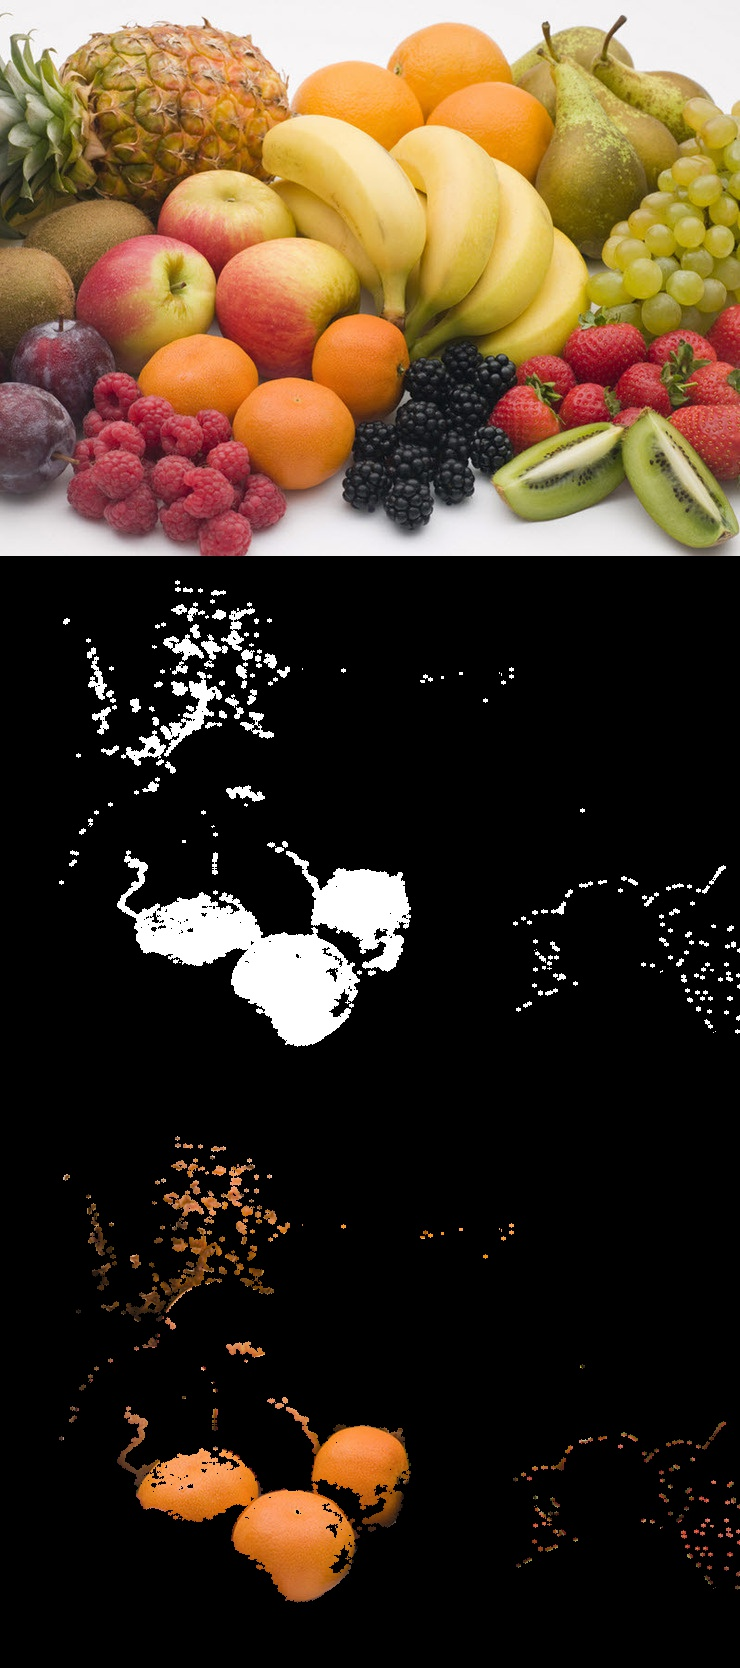
\includegraphics{res.jpg}

\hypertarget{additional-resources}{%
\subparagraph{Additional Resources}\label{additional-resources}}

``Indexing via color histograms'', Swain, Michael J. , Third
international conference on computer vision,1990.


    % Add a bibliography block to the postdoc
    
    
    
    \end{document}
